\documentclass{AsignaturaResumen}

\SetTitulo{Fenómenos de transporte}
    \def\ISMAIN{1}

% Glosario
    \setabbreviationstyle[acronym]{long-short}
\makeglossaries

    % Glosario

\newglossaryentry{polimorfismo}{
    name={Polimorfismo},
    description={Existencia de dos o más variantes (alelos) de una secuencia de ADN en una población}
}
\newglossaryentry{locus}{
    name={Locus},description={Posición que ocupa un gen en el cromosoma}}
\newglossaryentry{amplicones}{
    name={Amplicones},
    description={Secuencias de ADN producidas por la amplificación de la hebra original en una \acrshort{pcr}. Se identifican como las bandas de una electroforesis en gel}
}
\newglossaryentry{sucesion microbiana}{
    name={Sucesión microbiana},
    description={Evento donde las especies de microorganismos presentes en una muestran son reemplazadas por otras}
}
\newglossaryentry{variante de secuencia}{
    name={Variante de Secuencia de Amplicón},
    description={Amplicón único de un conjunto de secuencias obtenidas en una secuenciación ya corregida}
}
\newglossaryentry{homopolimero}{
    name={Homopolímero},
    description={Secuencia repetitiva de nucleótidos (AGTGCGAT\emph{AAAA}TGCAGT, p.e.)}
}

    % Acrónimos

\newacronym{si}{SI}{Sistema Internacional}
\newacronym{iubmb}{IUBMB}{Unión Internacional de Bioquímica y Biología Molecular}

\newacronym{ros}{ROS}{especies reactivas de oxígeno}

\newacronym{pb}{pb}{pares de bases}
\newacronym{kb}{kb}{kilobases}

\newacronym{adn}{ADN}{Ácido desoxirribonucléico}
\newacronym{adnc}{ADNc}{ADN complementario}
\newacronym{dntps}{dNTPs}{desoxirribonucleótidos trifosfato}
\newacronym{ddntps}{ddNTPs}{didesoxinucleótidos}

\newacronym{adnpol}{ADNpol}{ADN polimerasa}

\newacronym{pcr}{PCR}{Reacción en Cadena de la Polimerasa}
\newacronym{rapd}{RAPD}{ADN Polimórfico Amplificado al Azar}
\newacronym{rflp}{RFLP}{Fragmentos de Restricción de Longitud Polimórfica}
\newacronym{dpcr}{dPCR}{PCR digital}
\newacronym{ngs}{NGS}{Secuenciación de Nueva Generación}
\newacronym{smrt}{SMRT}{Secuenciación en Tiempo Real de Molécula Única}

\newacronym{ccs}{CCS}{Lecturas de Consenso Circular}
\newacronym{asv}{ASV}{Variante de Secuencia de Amplicón}

\newacronym{iqi}{IQI}{Índice de Calidad Infaunal}

\newacronym{sds}{SDS}{dodecilsulfato sódico}
\newacronym{dms}{DMS}{dimetilsulfato}
\newacronym{ctab}{CTAB}{bromuro de cetiltrimetilamonio}

\begin{document}

    \frontmatter

\Portada
\Indices

    \mainmatter

\part{Introducción a fenómenos de transporte}

    \chapter{Introducción a fenómenos de transporte} \ifx\ISMAIN\undefined
    \documentclass{AsignaturaResumen}
    \SetTitulo{Fenómenos de transporte}
    \setabbreviationstyle[acronym]{long-short}
\makeglossaries

    % Glosario

\newglossaryentry{polimorfismo}{
    name={Polimorfismo},
    description={Existencia de dos o más variantes (alelos) de una secuencia de ADN en una población}
}
\newglossaryentry{locus}{
    name={Locus},description={Posición que ocupa un gen en el cromosoma}}
\newglossaryentry{amplicones}{
    name={Amplicones},
    description={Secuencias de ADN producidas por la amplificación de la hebra original en una \acrshort{pcr}. Se identifican como las bandas de una electroforesis en gel}
}
\newglossaryentry{sucesion microbiana}{
    name={Sucesión microbiana},
    description={Evento donde las especies de microorganismos presentes en una muestran son reemplazadas por otras}
}
\newglossaryentry{variante de secuencia}{
    name={Variante de Secuencia de Amplicón},
    description={Amplicón único de un conjunto de secuencias obtenidas en una secuenciación ya corregida}
}
\newglossaryentry{homopolimero}{
    name={Homopolímero},
    description={Secuencia repetitiva de nucleótidos (AGTGCGAT\emph{AAAA}TGCAGT, p.e.)}
}

    % Acrónimos

\newacronym{si}{SI}{Sistema Internacional}
\newacronym{iubmb}{IUBMB}{Unión Internacional de Bioquímica y Biología Molecular}

\newacronym{ros}{ROS}{especies reactivas de oxígeno}

\newacronym{pb}{pb}{pares de bases}
\newacronym{kb}{kb}{kilobases}

\newacronym{adn}{ADN}{Ácido desoxirribonucléico}
\newacronym{adnc}{ADNc}{ADN complementario}
\newacronym{dntps}{dNTPs}{desoxirribonucleótidos trifosfato}
\newacronym{ddntps}{ddNTPs}{didesoxinucleótidos}

\newacronym{adnpol}{ADNpol}{ADN polimerasa}

\newacronym{pcr}{PCR}{Reacción en Cadena de la Polimerasa}
\newacronym{rapd}{RAPD}{ADN Polimórfico Amplificado al Azar}
\newacronym{rflp}{RFLP}{Fragmentos de Restricción de Longitud Polimórfica}
\newacronym{dpcr}{dPCR}{PCR digital}
\newacronym{ngs}{NGS}{Secuenciación de Nueva Generación}
\newacronym{smrt}{SMRT}{Secuenciación en Tiempo Real de Molécula Única}

\newacronym{ccs}{CCS}{Lecturas de Consenso Circular}
\newacronym{asv}{ASV}{Variante de Secuencia de Amplicón}

\newacronym{iqi}{IQI}{Índice de Calidad Infaunal}

\newacronym{sds}{SDS}{dodecilsulfato sódico}
\newacronym{dms}{DMS}{dimetilsulfato}
\newacronym{ctab}{CTAB}{bromuro de cetiltrimetilamonio}
    \begin{document}
    \chapter{Introducción a fenómenos de transporte}
\fi

Todo tipo de fenómeno de transporte se caracteriza por el funcionar en base al mismo tipo general de ecuación de transporte:

\begin{equation}
    \text{Velocidad de transporte molecular} = \frac{\text{Fuerza impulsora}}{\text{Resistencia}}
\end{equation}

Esto también se puede expresar como:

\begin{equation}\label{eq:ecuacion_de_transporte_molecular_diferencial}
    \Psi_{z} = \sigma\frac{\mathrm{d}\Gamma}{\mathrm{d}Z}
\end{equation}

Donde:

\begin{itemize}
    \item $\Psi_{z}$ es el flujo de propiedad, es decir, la cantidad de la propiedad que se transfiere por unidad de tiempo a través de una sección transversal unitaria perpendicular a la dirección del fljo en cantidad de propiedad dobre metro cuadrado.
    \item $\sigma$ es la difusividad en metro cuadrado sobre segundo (\unit{\m\squared\per\s}). Indica el gradiente y la resistencia
    \begin{itemize}
        \item La difusividad necesita de un gradiente para ocurrir.
    \end{itemize}
    \item $\Gamma$ es la concentración de la propiedad en cantidad de propiedad sobre metros cúbicos (\unit{\substance\per\m\cubed}). Indica la diferencia entre cantidad de transporte
    \item $Z$ es la distancia de la dirección del flujo en metros.
\end{itemize}

Si el proceso ocurre en un estado estacionario el flujo $\Psi_{z}$ es constante:

\begin{equation*}
    \Psi_{z} \ \mathrm{d}Z = - \sigma \ \mathrm{d}\Gamma
\end{equation*}

Esta es una ecuación diferencial que al resolverla por variables separables nos da:

\begin{equation}
    \Psi_{z} = \frac{-\sigma \ (\Gamma_{2} - \Gamma_{1})}{Z_{2} - Z_{1}}
\end{equation}


\resumebox{ejercicio}{Cálculo de flujo}{\footnotesize
    Se está transportando una propiedad por difusión a través de un fluido en estado estacionario. En un punto 1 determinado, la concentración es de \num{1.37d-2} cantidad de propiedad por metro cuadrado (\unit{\meter\squared}), y \num{0.72d-2} en el punto 2, a una distancia de \qty{0.4}{\m}. La difusividad es de \qty{0.013}{\m\squared\per\s}, y el área de corte transversal es constante.
    \begin{enumerate}
        \item Calcula el flujo
        \item Deduce la ecuación para $\Gamma$ como función de la distancia
        \item Calcule $\Gamma$ en el punto medio de la trayectoria
    \end{enumerate}
}

Al calcular las velocidades de transporte en un sistema usando la ecuación de transporte molecular (\autoref{eq:ecuacion_de_transporte_molecular_diferencial}) es necesario tomar en cuenta la cantidad de esta propiedad que se transporta en todo el sistema. Esto se hace escribiendo una ecuación general de balance o conservación para la propiedad en estado no estacionario.

\begin{align*}
    \text{Tasa de la propiedad que entra} \ &+ \ \text{Tasa de generación de la propiedad}
    \\
    &=
    \\
    \text{Tasa de la propiedad que sale} \ &+ \ \text{Tasa de acumulación de la propiedad}
\end{align*}

La velocidad de entrada es $\Psi_{Z / (Z \cdot 1)}$ en cantidad de propiedad sobre segundo (\unit{\substance\per\s}), mientras que la velocidad de salida es $(\Psi_{Z/Z} + \Delta Z) \cdot 1$ en cantidad de propiedad sobre segundo , donde el área de corte transversal es de \qty{1}{\m\squared}. La velocidad de generación de la propiedad se escribe como $R_{\Delta Z \cdot 1}$, que se mide en cantidad de propiedad sobre segundo por metro cúbico (\unit{\substance\per\m\cubed\per\s}). El término para la acumulación es:

\begin{equation}
    \text{Velocidad de acumulación de propiedad} = \frac{\mathrm{d}\Gamma (\Delta Z \cdot 1)}{\mathrm{d}t} 
\end{equation}

En la cual, si sustituimos, tendríamos:

\begin{equation}
    \Psi_{Z / (Z \cdot 1)} + R_{\Delta Z \cdot 1} = (\Psi_{Z/Z} + \Delta Z) \cdot 1 + \frac{\mathrm{d}\Gamma}{\mathrm{d}t} (\Delta Z \cdot 1)
\end{equation}


\section{Tipos de transporte}

\subsection{Transporte de momento lineal y la ley de Newton}

\resumebox{definicion}{Primera Ley de Newton}{\footnotesize
    Todo cuerpo persevera en su estado de reposo o movimiento uniforme y rectilíneo a no ser que sea obligado a cambiar su estado por fuerzas impresas sobre él.
}

Cuando un fluido fluye en la dirección X en forma paralela a una superficie sólida existe un gradiente de velocidad dondel a velocidad $V_{x}$ en la dirección X disminuye al acercarse a la superficie en la dirección z. El fluido tiene un momento lineal en dirección X y su concentración es $V_{x}\rho$ (momento lineal sobre metro cúbico), donde el momento lineal tiene unidades de kilogramos por metro sobre segundo (\unit{\kg\m\per\s}). Debido a la difusión aleatoria de las moléculas existe un intercambio de moléculas en la dirección z, moviendose igual número de ellas en cada dirección entre la capa de la molécula que se mueve más rápido y la capa adyacente más lenta. La ley que describe lo anterior es la ley de Newton de la viscosidad para una densidad constante:

\begin{equation}
    \tau_{zx} = -\nu \cdot \frac{\mathrm{d}(\rho \cdot V_{x})}{\mathrm{d}z}
\end{equation}

Donde:

\begin{itemize}
    \item $\tau_{zx}$ es el flujo de momento lineal con dirección X en la dirección Z (\unit{\kg\m\per\s})
    \item $V$ es $\frac{\mu}{\rho}$, que representa la difusividad de momento lineal en metro cuadrado por segundo (\unit{\m\squared\per\s})
    \item $z$ es la dirección de transporte o difusión en metros (\unit{\m})
    \item $\rho$ es la densidad en kilogramos por metro cúbico (\unit{\kg\per\m\cubed})
    \item $\mu$ es la viscosodad en kilogramos por metro por segundo (\unit{\kg\per\m\s})
\end{itemize}

\subsection{Transporte de calor y la ley de Fourier}

La ley de Fourier para el transporte molecular de calor o la conducción de calor en un fluido o sólido puede escribirse para una densidad constante y capacidad calorífica (cp) de la siguiente manera:

\begin{equation}
    \frac{qz}{A} = -\alpha \cdot \frac{\mathrm{d}(\rho \cdot \unit{\cp} \cdot T)}{\mathrm{d}z}
\end{equation}

Donde:

\begin{itemize}
    \item $\frac{qz}{A}$ es el flujo de calor en \unit{\joule\per\m\squared\s}
    \item $\alpha$ es la difusividad térmica en \unit{\m\squared\per\s}
    \item $\rho \cdot \unit{\cp} \cdot T$ es la concentración de calor o energía térmica en \unit{\joule\per\m\cubed}
\end{itemize}

Cuando hay un gradiente de temperatura en un fluido se difunden igual número de moléculas entre la región caliente y la más fría.

\subsection{Transporte de masa y ley de Fick}

La ley de Fick para el transporte molecular de masa en un fluido o en un sólido para la concentración total constante del fluido es:

\begin{equation}
    J_{AZ} = -D_{AB} \cdot \frac{\mathrm{d}C_{A}}{\mathrm{d}Z}
\end{equation}

Donde:

\begin{itemize}
    \item $J_{AZ}$ es el flujo de A en kgmol de A sobre \unit{\m\squared\s}
    \item $D_{AB}$ es la difusividad molecular de las moléculas A y B en \unit{\m\squared\per\s}
    \item $C_{A}$ es la concentración de A en \unit{\kg\mole} de A sobre \unit{\m\cubed} (\unit{\kg\mole\per\m\cubed})
\end{itemize}

Donde existe un gradiente de concentración en un fluido se difundirán igual número de moléculas en todas las direcciones de alta y baja concentración, y ocurrirá un flujo neto de masa.



% -------------------------------------------------------------------- %

\section{Respuestas de ejercicios}

\resumebox{respuesta}{Cálculo de flujo}{
\begin{enumerate}
\item Calculo del flujo:
\begin{gather*}
    \Psi_{z} = - \frac{\delta (\Gamma_{2} - \Gamma_{1})}{Z_{2} - Z_{1}}
    \\
    \Psi_{z} = - \frac{ \qty{0.013}{\m\squared\per\s} \cdot \left( \qty{1.37d-2}{\substance\per\m\cubed} - \qty{0.72d-2}{\substance\per\m\cubed} \right) }{\qty{0.4}{\m}} = \qty{2.1125d-4}{\substance\per\m\squared\per\s}
\end{gather*}
\item Ecuación para $\Gamma$ como función de la distancia:
\begin{equation*}
     \Psi_{z} = - \frac{\delta (\Gamma_{2} - \Gamma_{1})}{Z_{2} - Z_{1}} 
     \quad\longrightarrow\quad
     \Gamma = \frac{\Psi_{z} \cdot Z}{-\delta}
\end{equation*}
\item $\Gamma$ en el punto medio:
\begin{gather*}
    \Gamma_{\qty{0.2}{\m}} = \frac{ \qty{2.1125d-4}{\substance\per\m\squared\per\s} \cdot \qty{0.2}{\m} }{ \qty{0.013}{\m\squared\per\s} } - \qty{1.37d-2}{\substance\per\m\cubed}
    \\
    \Gamma_{\qty{0.2}{\m}} = \qty{1.045d-2}{\substance\per\m\cubed}
\end{gather*}
\end{enumerate}
}

\ifx\ISMAIN\undefined
    \end{document}
\fi

\part{Transporte de momento}

    \chapter{Presión en fluidos} \ifx\ISMAIN\undefined
    \documentclass{AsignaturaResumen}
    \SetTitulo{Fenómenos de transporte}
    \setabbreviationstyle[acronym]{long-short}
\makeglossaries

    % Glosario

\newglossaryentry{polimorfismo}{
    name={Polimorfismo},
    description={Existencia de dos o más variantes (alelos) de una secuencia de ADN en una población}
}
\newglossaryentry{locus}{
    name={Locus},description={Posición que ocupa un gen en el cromosoma}}
\newglossaryentry{amplicones}{
    name={Amplicones},
    description={Secuencias de ADN producidas por la amplificación de la hebra original en una \acrshort{pcr}. Se identifican como las bandas de una electroforesis en gel}
}
\newglossaryentry{sucesion microbiana}{
    name={Sucesión microbiana},
    description={Evento donde las especies de microorganismos presentes en una muestran son reemplazadas por otras}
}
\newglossaryentry{variante de secuencia}{
    name={Variante de Secuencia de Amplicón},
    description={Amplicón único de un conjunto de secuencias obtenidas en una secuenciación ya corregida}
}
\newglossaryentry{homopolimero}{
    name={Homopolímero},
    description={Secuencia repetitiva de nucleótidos (AGTGCGAT\emph{AAAA}TGCAGT, p.e.)}
}

    % Acrónimos

\newacronym{si}{SI}{Sistema Internacional}
\newacronym{iubmb}{IUBMB}{Unión Internacional de Bioquímica y Biología Molecular}

\newacronym{ros}{ROS}{especies reactivas de oxígeno}

\newacronym{pb}{pb}{pares de bases}
\newacronym{kb}{kb}{kilobases}

\newacronym{adn}{ADN}{Ácido desoxirribonucléico}
\newacronym{adnc}{ADNc}{ADN complementario}
\newacronym{dntps}{dNTPs}{desoxirribonucleótidos trifosfato}
\newacronym{ddntps}{ddNTPs}{didesoxinucleótidos}

\newacronym{adnpol}{ADNpol}{ADN polimerasa}

\newacronym{pcr}{PCR}{Reacción en Cadena de la Polimerasa}
\newacronym{rapd}{RAPD}{ADN Polimórfico Amplificado al Azar}
\newacronym{rflp}{RFLP}{Fragmentos de Restricción de Longitud Polimórfica}
\newacronym{dpcr}{dPCR}{PCR digital}
\newacronym{ngs}{NGS}{Secuenciación de Nueva Generación}
\newacronym{smrt}{SMRT}{Secuenciación en Tiempo Real de Molécula Única}

\newacronym{ccs}{CCS}{Lecturas de Consenso Circular}
\newacronym{asv}{ASV}{Variante de Secuencia de Amplicón}

\newacronym{iqi}{IQI}{Índice de Calidad Infaunal}

\newacronym{sds}{SDS}{dodecilsulfato sódico}
\newacronym{dms}{DMS}{dimetilsulfato}
\newacronym{ctab}{CTAB}{bromuro de cetiltrimetilamonio}
    \begin{document}
    \chapter{Presión en fluidos}
\fi

%\section{Ecuaciones para el balance de movimiento}



\section{Presión}\label{sec:presion}

Si se requiere calcular la cantidad de kg totales de un fluido se utiliza:

\begin{equation*}
    kg_{\text{Total}} = h_{2}(m) \cdot A(m^{2}) \cdot \rho(kg/m^{2}) = h_{2} \cdot A \cdot \rho_{g} 
\end{equation*}

Para calcular la fuerza total ($F$) del fluido sobre el área 1 debido unicamente al fluido es:

\begin{equation}
    F = (h_{2} \cdot A \cdot P)(g)
\end{equation}

\begin{equation}
    P = \frac{F}{A} \quad\therefore\quad P = h_{2} \cdot \rho_{g}
\end{equation}

Esta es la presión sobre A\sub{2} debido a la masa del fluido que está encima. Sin embargo, para obtener la presión total (P\sub{2}) sobre A\sub{2}debe añadirse P\sub{0}, que soporta todo el líquido, de tal manera que:

\begin{equation}
    F = h_{2} \cdot \rho_{g} + P_{0}
\end{equation}

Esta ecuación es la expresión fundamental para calcular la presión de un fluido a cualquier profundidad.

Para P\sub{1}:

\begin{equation}
    P_{1} = h_{1} \cdot \rho_{g} + P_{0}
\end{equation}

La diferencia entre los dos puntos es:

\begin{equation}
    P_{2} - P_{1} = (h_{2} \cdot \rho_{g} + P_{0}) - (h_{1} \cdot \rho_{g} + P_{0})
\end{equation}

\resumebox{ejercicio}{Calculo de presión}{\footnotesize
    Un gran tanque de almacenamiento contiene petroleo de una densidad igual a \qty{917}{\kg\per\m\cubed}. El tanque tiene una altura de \qty{3.66}{\m} y está abierto a la atmósfera con una presión de 1atm absoluta en la superficie. El tanque está lleno con petroleo a una profundidad de \qty{3.05}{\m} y contiene tambien \qty{0.61}{\m} de agua en la parte inferior. calcule la presión en pascales a \qty{3.05}{\m} de la superficie y en el fondo del tanque. También calcule la presión manométrica del fondo del tanque.
    \begin{figure}[H]
        \centering
        \resizebox{0.45\linewidth}{!}{\begin{tikzpicture}[
    principal/.style={line width=1pt},
    trasera/.style={dashed, line width=1pt},
    flecha/.style={|-Stealth},
    delimitador/.style={|-|, line width=0.75pt},
    texto/.style={font=\sffamily}
]

\draw[principal] (2.5,-2.5) -- (-2.5,-2.5) -- node[pos=0.4] (esq4) {} (-2.5,2.5) -- (2.5,2.5) -- node[pos=0.6] (esq3) {} (2.5,-2.5);
\draw[principal] (-5,0) -- node[pos=0.4] (esq1) {} (-5,5) -- (0,5);
\draw[principal] (-5,5) -- (-2.5,2.5);
\draw[principal] (-5,0) -- (-2.5,-2.5);
\draw[principal] (2.5,2.5) -- (0,5);

\draw[trasera] (0,5) -- node[pos=0.6] (esq2) {} (0,0) -- (-5,0);
\draw[trasera] (0,0) -- (2.5,-2.5);

\draw[trasera] (esq1) -- (esq2) -- (esq3) -- (esq4) -- (esq1);

\draw[delimitador] (3.5,2.5) -- (3.5,0) node[midway, left=0pt, texto] {h$_{1}$};
\draw[delimitador] (3.5,0) -- (3.5,-2.5) node[midway, left=0pt, texto] {h$_{3}$};
\draw[delimitador] (4.5,2.5) -- (4.5,-2.5) node[midway, left=0pt, texto] {h$_{2}$};


\draw[flecha] (-6,4) node[texto, left=0pt] {A$_{0}$} -- (-3.25,4);
\draw[flecha] (-6,1.25) node[texto, left=0pt] {A$_{1}$} -- (-3.25,1.25);
\draw[flecha] (-6,-0.75) node[texto, left=0pt] {A$_{2}$} -- (-3.25,-0.75);

\draw[flecha] (-0.8,6) -- (-0.8,3.75) node[texto, pos=0.8, right=0pt] {P$_{0}$};
\draw[flecha] (-0.8,3.5) -- (-0.8,0.5) node[texto, pos=0.8, right=0pt] {P$_{1}$};
\draw[flecha] (-0.8,0.25) -- (-0.8,-1.75) node[texto, pos=0.7, right=0pt] {P$_{2}$};
\end{tikzpicture}}
        \rule{\linewidth}{0.5pt}
        \caption{Diagrama del tanque}
    \end{figure}
}


\section{Viscosidad} % Ley de Newton y viscosidad

Cuando un fluido se transporta a través de un canal cerrado se presentan dos tipos de flujo dependiendo de dicho fluido:

\begin{enumerate}
    \item A \emph{velocidades bajas} el fluido tiende a transportarse sin mezclado lateral, y las capas adyacentes se resbalan unas sobre las otras. En este caso no hay corrientes cruzadas perpendiculares a la dirección del flujo, ni tampoco remolinos de fluidos. A este tipo de flujo se le llama \emph{flujo laminar}.
    \item A \emph{velocidades altas} se forman remolinos, lo que conduce a un mezclado lateral. A este tipo de flujo se le llama \emph{flujo turbulento}.
\end{enumerate}

La viscosidad es una propiedad de un fluido que da lugar a fuerzas que se oponen al movimiento relativo de capas adyacentes en el fluido. Para muchos fluidos se ha determinado de forma experimental que la fuerza (F) en Newtons es directamente proporcional a la velocidad $\Delta V_{z}$ en metros sobre segundo (\unit{\m\per\s}). El área en metros cuadrados (\unit{\m\squared}) de la placa usada es inversamente proporcional a la distancia $\Delta y$ en metros (\unit{\m}). Expresada con la ley de viscosidad de Newton, cuando el flujo es laminar:

\begin{equation}
    \frac{F}{A} = -\mu \frac{\Delta V_{z}}{\Delta y}
\end{equation}

Donde $\mu$ es la constante de proporcionalidad llamada viscosidad del fluido en pascales por segundo (\unit{\pascal\s}) o \unit{\kg\per\m\s}. Cuando $\Delta y$ tiende a 0:

\begin{equation}
    \tau_{yz} = -\mu \cdot \frac{dV_{z}}{dy}
\end{equation}

\begin{equation}\footnote{lbf/ft\super{2}}
    \tau_{yz} \ gc = -\mu \cdot \frac{dV_{z}}{dy}
\end{equation}

Las unidades en el \emph{sistema cgs} son \unit{\g\m\per\s}, llamados Poise (P) o Centipoise (cp). 

\resumebox{ejercicio}{Cálculo de esfuerzo cortante}{\footnotesize
    La distancia entre las dos placas es de \qty{0.5}{\cm}. La velocidad de flujo que pasa a través es de \qty{10}{\cm\s}, y el fluido que atraviesa se trata de alcohol etílico a \qty{273}{\K}, cuya viscosidad es de \qty{1.77}{cp}.
    \begin{enumerate}
        \item Calcule el esfuerzo cortante $\tau_{yz}$ y el gradiente de velocidad
        \item Repita en SI
    \end{enumerate}
}

\section{Fluidos newtonianos y no newtonianos}

\marginpar{\begin{minipage}{\marginparwidth}
\begin{figure}[H]
    \centering
    \resizebox{\linewidth}{!}{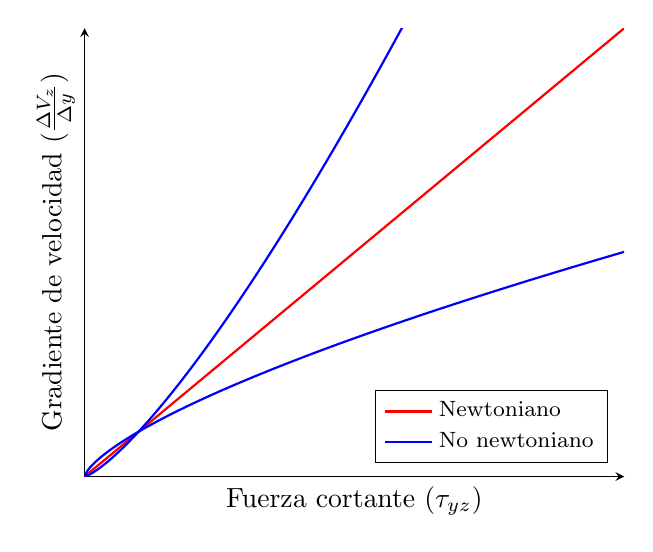
\begin{tikzpicture}
\begin{axis}[
    axis lines = left,
    ticks = none,
    xmin=0, xmax=10,
    ymin=0, ymax=10,
    xlabel = {Fuerza cortante ($\tau_{yz}$)},
    ylabel = {Gradiente de velocidad ($\frac{\Delta V_{z}}{\Delta y}$)},
    domain=0:10, 
    samples=200,
    legend pos = south east,
    legend cell align = left
]
    \addplot[thick, color=red]{x};
    \addlegendentry{\footnotesize Newtoniano}
    \addplot[thick, color=blue]{x^0.7};
    \addplot[thick, color=blue]{x^1.3};
    \addlegendentry{\footnotesize No newtoniano}
\end{axis}
\end{tikzpicture}}
    \rule{\linewidth}{0.5pt}
    \caption{Diferencia entre fluidos newtonianos y no newtonianos}
    \label{fig:grafica_de_tipos_de_fluidos}
\end{figure}
\end{minipage}}

Los fluidos que obedecen la ley de viscosidad e Newton se les llama fluidos newtonianos. En dichos fluidos existe una relación lineal entre el esfuerzo cortante ($\tau_{yz}$) y el gradiente de velocidad ($\frac{\Delta V_{z}}{\Delta y}$), lo cual significa que la velocidad $\mu$ es constante e independiente de la velocidad cortante. En fluidos no newtonianos, la relación entre $\tau_{yz}$ y $\frac{\Delta V_{z}}{\Delta y}$ no es lineal, es decir, $\mu$ no permanece constante, sino que está en función de $\tau_{yz}$.

La viscosidad de los gases, que son fluidos newtonianos, aumenta con la temperatura e independiente de la presión.




% -------------------------------------------------------------------- %

\section{Respuestas de ejercicios}

\resumebox{respuesta}{Calculo de presión}{
\begin{gather*}
    \mathrm{1atm} = \qty{1.01325d5}{\pascal} 
    \quad;\quad
    \unit{\pascal} = \frac{\unit{\kg\m\per\s\squared}}{\unit{\m\squared}} = \unit{\kg\per\m\per\s\squared}
%    \mathrm{P_{n}} = (h_{n} \cdot \rho_{n} \cdot g) + P_{n-1}
    \\\\
    \mathrm{P_{Petroleo}} = \left( \qty{3.05}{\m} \cdot \qty{917}{\kg\per\m\cubed} \cdot \qty{9.81}{\m\per\s\squared} \right) + \qty{1.01325d5}{\kg\per\s\squared\per\m} = \qty{1.2876d5}{\pascal}
    \\
    \mathrm{P_{Agua}} = \left( \qty{0.61}{\m} \cdot \qty{1000}{\kg\per\m\cubed} \cdot \qty{9.81}{\m\per\s\squared} \right) + \qty{1.2876d5}{\kg\per\s\squared\per\m} = \qty{1.3474d5}{\pascal}
    \\
    \mathrm{P_{Fondo (Manométrica)}} = \qty{1.3474d5}{\pascal} - \qty{1.2876d5}{\pascal} = \qty{33415}{\pascal} = \qty{33.415}{\kilo\pascal}
\end{gather*}
}

\resumebox{respuesta}{Cálculo de esfuerzo cortante}{\footnotesize
\begin{enumerate}
\item Calcule el esfuerzo cortante $\tau_{yz}$ y el gradiente de velocidad
\begin{gather*}
    V = \qty{10}{\cm\per\s} 
    \quad;\quad
    \mu = \qty{1.77}{\cp} = \qty{1.777d-3}{\P}
    \quad;\quad 
    y = \qty{0.5}{\cm}
    \\
    \tau_{yz} = \qty{1.77d-2}{\P} \cdot \frac{\qty{10}{\cm\per\s}}{\qty{0.5}{\cm}} = \qty{0.354}{\pascal\s}
    \\
    \frac{\Delta V_{z}}{\Delta y} = \frac{\qty{10}{\cm\per\s}}{\qty{0.5}{\cm}} = \qty{20}{\per\s}
\end{gather*}
\item Repita en SI
\begin{gather*}
    V = \qty{0.1}{\m\per\s} 
    \quad;\quad
    \mu = \qty{1.77d-3}{\pascal\s}
    \quad;\quad
    y = \qty{0.005}{\m}
    \\
    \tau_{yz} = \qty{1.77d-3}{\pascal\s} \cdot \frac{\qty{0.1}{\m\per\s}}{\qty{0.005}{\m}} = \qty{3.54d-2}{\pascal}
%   \\\\
%   \frac{\Delta V_{z}}{\Delta y} = \frac{\qty{10}{\cm\per\s}}{\qty{0.5}{\cm}} = \qty{20}{\per\s}
\end{gather*}
\end{enumerate}
}


\ifx\ISMAIN\undefined
    \end{document}
\fi
    \chapter{Transferencia de momento lineal} \ifx\ISMAIN\undefined
    \documentclass{AsignaturaResumen}
    \SetTitulo{Fenómenos de transporte}
    \setabbreviationstyle[acronym]{long-short}
\makeglossaries

    % Glosario

\newglossaryentry{polimorfismo}{
    name={Polimorfismo},
    description={Existencia de dos o más variantes (alelos) de una secuencia de ADN en una población}
}
\newglossaryentry{locus}{
    name={Locus},description={Posición que ocupa un gen en el cromosoma}}
\newglossaryentry{amplicones}{
    name={Amplicones},
    description={Secuencias de ADN producidas por la amplificación de la hebra original en una \acrshort{pcr}. Se identifican como las bandas de una electroforesis en gel}
}
\newglossaryentry{sucesion microbiana}{
    name={Sucesión microbiana},
    description={Evento donde las especies de microorganismos presentes en una muestran son reemplazadas por otras}
}
\newglossaryentry{variante de secuencia}{
    name={Variante de Secuencia de Amplicón},
    description={Amplicón único de un conjunto de secuencias obtenidas en una secuenciación ya corregida}
}
\newglossaryentry{homopolimero}{
    name={Homopolímero},
    description={Secuencia repetitiva de nucleótidos (AGTGCGAT\emph{AAAA}TGCAGT, p.e.)}
}

    % Acrónimos

\newacronym{si}{SI}{Sistema Internacional}
\newacronym{iubmb}{IUBMB}{Unión Internacional de Bioquímica y Biología Molecular}

\newacronym{ros}{ROS}{especies reactivas de oxígeno}

\newacronym{pb}{pb}{pares de bases}
\newacronym{kb}{kb}{kilobases}

\newacronym{adn}{ADN}{Ácido desoxirribonucléico}
\newacronym{adnc}{ADNc}{ADN complementario}
\newacronym{dntps}{dNTPs}{desoxirribonucleótidos trifosfato}
\newacronym{ddntps}{ddNTPs}{didesoxinucleótidos}

\newacronym{adnpol}{ADNpol}{ADN polimerasa}

\newacronym{pcr}{PCR}{Reacción en Cadena de la Polimerasa}
\newacronym{rapd}{RAPD}{ADN Polimórfico Amplificado al Azar}
\newacronym{rflp}{RFLP}{Fragmentos de Restricción de Longitud Polimórfica}
\newacronym{dpcr}{dPCR}{PCR digital}
\newacronym{ngs}{NGS}{Secuenciación de Nueva Generación}
\newacronym{smrt}{SMRT}{Secuenciación en Tiempo Real de Molécula Única}

\newacronym{ccs}{CCS}{Lecturas de Consenso Circular}
\newacronym{asv}{ASV}{Variante de Secuencia de Amplicón}

\newacronym{iqi}{IQI}{Índice de Calidad Infaunal}

\newacronym{sds}{SDS}{dodecilsulfato sódico}
\newacronym{dms}{DMS}{dimetilsulfato}
\newacronym{ctab}{CTAB}{bromuro de cetiltrimetilamonio}
    \begin{document}
    \chapter{Transferencia de momento lineal}
\fi


\section{Tipos de flujo}

El primer tipo de flujo ocurre a velocidades bajas, donde la capa del fluido parece desplazarse unas sobre las otras sin remolinos o turbulencias. Tal flujo se llama flujo laminar, y obedece la ley de la viscosidad de Newton.

El segundo tipo de flujo ocurre avelocidades más altas, donde se forman remolinos que imparten al fluido una naturaleza fluctante. Este fluido recibe el nombre de flujo turbulento. 

\section{Número de Reynolds (N\sub{Re})}

La expresión para estimar el número de Reynolds es:

\begin{equation}\label{eq:numero_de_reynolds}
\mathrm{ N_{Re} = \frac{D \cdot V \cdot \rho}{\mu} }\end{equation}

Aquí D es el diametro de la tubería en metros (\unit{\m}). V es la velocidad promedio del fondo en metros por segundo (\unit{\m\per\s}), y se obtiene con la velocidad volumétrica del fluida dividida entre el área de corte transversal de la tubería.

Cuando N\sub{Re} es menor a 2100 para una tubería circular recta, el flujo siempre es laminar. Cuand el valor supera 4000 el flujo será turbulento. Entre estos dos valores está la \emph{región de transición}, en la cual el flujo puede ser laminar o turbulento dependiendo de detalles del sistema que no se pueden predecir.

\begin{align*}
    \mathrm{N_{Re}} < 2100        &\quad\longrightarrow\quad \text{Flujo laminar}
    \\
    2100 < \mathrm{N_{Re}} < 4000 &\quad\longrightarrow\quad \text{Región de transición}
    \\
    \mathrm{N_{Re}} > 4000        &\quad\longrightarrow\quad \text{Flujo turbulento}
\end{align*}

\marginpar{\resumebox{ejercicio}{Número de Reynolds}{\footnotesize
    Por una tubería con un diámetro interior de \qty{2.007}{\in} fluye agua a \qty{303}{\K} con una velocidad de \qty{10}{\gal\per\min}.
Calcular el N\sub{Re} usando unidades del sistema internacional 
}}


\section{Balance general de momento lineal}

La ecuación para la conservación del momento lineal con respecto a un volumen de control se puede describir como:

\begin{equation*}
    \sum{\text{Fuerzas}} = V_{\text{Salida}} - V_{\text{Entrada}} + V_{\text{Acumulación}}
\end{equation*}

Siendo $V$ la velocidad de momento lineal. Este momento lineal no se conserva ya que es generado por fuerzas externas. Si no existen fuerzas externas entonces si hay conservación de momento lineal

\section{Ecuación de diseño para flujo laminar y turbulento en tuberías}

Una de las aplicaciones más importantes del transporte de fluidos es el flujo en conductos circulares, tuberías y caños. Cuando el fluido pasa a través de una tubería circular, al medir la velocidad a diferentes distancias de la pared al centro el fluido que está en el centro del tubo se desplaza con mayor rapidez que el que está cercano a la tubería o pared.

\section{Caida de presión y pérdida por fricción en un flujo laminar}

Cuando un líquido o gas fluyen por una tubería con flujo laminar en estado estacionario, la ecuación se escribe para variaciones de radio ($dr$) en vez de la distancia:

\begin{equation}
    \tau_{yz} = -\mu \cdot \frac{dV_{s}}{dr}
\end{equation}

Con esta ecuación y llevando a cabo un balance de momento lineal en un recinto cilíndrico se obtiene la ecuación de Hagen-Poiseville:

\begin{equation}
    \Delta P_{f} = (P_{1} - P_{2})_{f} = \frac{32\mu \cdot V \cdot \Delta L}{D^{2}}
\end{equation}

Donde:
\begin{itemize}
    \item $P_{1}$ es la presión corriente arriba en el punto 1
    \item $P_{2}$ es la presión corriente arriba en el punto 2
    \item $V$ es la velocidad promedio en el tubo
    \item $D$ es el diametro interno
    \item $\Delta L$ es la longitud del tubo
\end{itemize}

Para el sistema inglés es:

\begin{equation*}
    \Delta P_{f} = (P_{1} - P_{2})_{f} = \frac{32\mu \cdot V \cdot \Delta L}{D^{2} \cdot gc}
\end{equation*}

Para una presión constante, la pérdida por presión ($F_{f}$) se puede calcular de la siguiente manera:

\begin{equation}
    F_{f} = \frac{(P_{1} - P_{2})_{f}}{P}
\end{equation}

\resumebox{ejercicio}{Cálculo de flujo másico}{
    Para medir en forma continua la velocidad del flujo de un líquido con una densidad de \qty{875}{\kg\per\m\cubed} y una viscosidad de \qty{1.13d-3}{\pascal\s} se usa un pequeño capilar con un diametro interno de \qty{2.22d-3}{\m} y la longitud igual a \qty{0.317}{\m}. La lectura de caida de presión es de \qty{0.0655}{\m} de agua, la cual tiene una densidad de \qty{996}{\kg\per\m\cubed}. ¿Cuál es la velocidad de flujo en \unit{\m\cubed\per\s} sin tomar en cuenta los efetos de los extremos del tubo?
}

\section{Factor de fricción de Fanning ($f$)}

Un parámetro muy común en el flujo laminar es el factor de fricción de Fanning ($f$), que se define como la fuerza de arrastre por unidad de área --- dividida entere el prducto de la densidad por la carga de velocidad, o altura dinámica. La fuerza es $\Delta P_{f}$ multiplicada por el área de sección transversal y el área de superficie mojada. La relación entre la caída de presión debida a la fricción es la siguiente para flujo laminar y turbulento:

\begin{equation}
    f = \frac{\tau_{s}}{\rho \cdot (V^{2} \div 2)} = \frac{\Delta P_{f} \cdot \pi \cdot R \cdot \rho \cdot V^{2}}{2\pi \cdot R \cdot \Delta L}
\end{equation}

\begin{equation}
    \Delta P_{f} = \frac{4f \cdot \rho \cdot \Delta L \cdot V^2}{2D} \quad;\quad \Delta P_{f(\text{Inglés})} = \frac{4f \cdot \rho \cdot \Delta L \cdot V^2}{2D \cdot gc}
\end{equation}

\begin{equation}
    F_{f} = \frac{\Delta P_{f}}{\rho} = \frac{4f \cdot \Delta L \cdot V^2}{2D} \quad;\quad F_{f(\text{Inglés})} = \frac{4f \cdot \Delta L \cdot V^2}{2D \cdot gc}
\end{equation}

\begin{equation}
    \text{Laminar:} f = \frac{16}{\mathrm{N_{Re}}} \quad;\quad \text{Turbulento:} f = \frac{0.0791}{\mathrm{N_{Re}}^{0.25}}
\end{equation}


\resumebox{ejercicio}{Cálculo de caida de presión}{\footnotesize
    Suponga las mismas condiciones conocidas del ejemplo anterior, excepto que se conoce la velocidad, que es de \qty{0.225}{\m\per\s}, y se debe pronosticar la caida de presión. Use el método de factor de fricción de Fanning ($F_{f}$)
}

\resumebox{ejercicio}{Cálculo de pérdida por fricción}{\footnotesize
    Un líquido fluye por una tubería horizontal recta de acero comercial a \qty{4.57}{\m\per\s}. El diámetro interno de la tubería es de \qty{2.067}{\in}, mientras que la viscosidad del líquido es de \qty{4.46}{\cp}, y su densidad es de \qty{801}{\kg\per\m\cubed}. Calcule la pérdida por fricción de energía mecánica (F\sub{f}) en \unit{\J\per\kg} para una sección de tubería de \qty{36.6}{\m}.
}

\resumebox{ejercicio}{Cálculo de caida de presión por efectos de fricción}{\footnotesize
    Calcule la caida de presión por efectos de la fricción, expresada en \unit{\pascal}, para un aceite de ilivo a \qty{293}{\K}, que fluye por una tubería comercial de diametro interno igual a \qty{0.0525}{\m} y una lngiud de \qty{76.2}{\m}. La velocidad de fluido es de \qty{1.22}{\m\per\s}.Utilice el método del factor de fricción.
    \begin{enumerate}
        \item ¿Es el flujo laminar o turbulento si la densidad del medio es de \qty{919}{\kg\per\m\cubed} y su viscosidad de \qty{8.4d-2}{\kg\per\m\per\s}?
        \item ¿Cuál sería el valor de fricción si se cambia el aceite por otro que tenga una viscosidad de \qty{8.4d-4}{\kg\per\m\per\s} y todo lo demás se conserva igual?
    \end{enumerate}
}

\resumebox{ejercicio}{Cálculo de pérdida por fricción $F_{f}$}{\footnotesize
    Un líquido con densidad de \qty{801}{\kg\per\m\cubed} y visosidad de \qty{1.49d-3}{\pascal\s} fluye por una tubería horizontal recta a velocidad de \qty{4.57}{\m\per\s}. El tubo de acero comercial es de tamaño nominal de \qty{1.5}{\in}, cédula 40. Proceda a lo siguiente para un tubo de \qty{61}{\m} de largo:
    \begin{enumerate}
        \item Calcule la pérdida por fricción $F_{f}$
        \item Calcule la pérdida por fricción de una tubería lisa del mismo diametro interior, ¿cuál es el porcentaje de reducción de $F_{f}$ para una tubería lisa?
    \end{enumerate}
}

\resumebox{ejercicio}{Cálculo de velocidad de flujo}{\footnotesize
    En un proyecto hidráulico se diagrama una tubería de hierro \emph{colado} de \qty{0.156}{\m} de diametro interior y \qty{305}{\m} de longitud, para drenar aguas negras a \qty{293}{\K}. La carga disponible es de \qty{4.57}{\m} de agua. Despreciando las pérdidas en los acesorios y conexiones de la tubería, calcule la velocidad de flujo en \unit{\m\cubed\per\s}. \\
    \emph{Sugerencia:} Suponga las propiedades del agua pura, la solución se logra por prueba y error, pues N\sub{Re}, que es necesario para calcular el factor de fricción que depende de la velocidad. Como primera aproximación, suponga que la velocidad es de \qty{1.7}{\m\per\s}. \\
    La densidad del líquido es de \qty{998.2}{\kg\per\m\cubed} y la visocisdad es de \qty{1.005d-3}{\kg\per\m\per\s}.
}


%\section{Ecuación de Bernoulli}
%    \begin{equation}
%        P_{1} + \frac{1}{2} \rho v_{1}^{2} + \rho g h_{1} = P_{2} + \frac{1}{2} \rho v_{2}^{2} + \rho g h_{2}
%    \end{equation}
%\section{Ecuación de continuidad para flujo unidireccional y en punto}





% -------------------------------------------------------------------- %

\section{Respuestas de ejercicios}

\resumebox{respuesta}{Número de Reynolds}{
\begin{gather*}
    \mathrm{D} = \qty{2.007}{\in} \cdot \qty{2.54}{\cm\per\in} \cdot \frac{\qty{1}{\m}}{\qty{100}{\cm}}= \qty{5.1d-2}{\m}
    \\
    \mathrm{V_{Volumétrica}} = \qty{10}{\gal\per\min} \cdot \frac{\qty{1}{\min}}{\qty{60}{\s}} \cdot \qty{3.7854d-3}{\m\cubed\per\gal} = \qty{6.309d-4}{\m\cubed\per\s}
    \\
    V = \frac{\qty{6.309d-4}{\m\cubed\per\s}}{\pi \cdot (\qty{5.1d-2}{\m} \div 2)^{2}} = \qty{0.3088}{\m\per\s}
    \\
    \mu = \qty{0.8007}{\cp} \cdot \frac{\qty{1d-3}{\kg\per\m\s}}{1cp} = \qty{8.007d-4}{\kg\per\m\per\s}
    \\
    \mathrm{N_{Re}} = \frac{\qty{5.1d-2}{\m} \cdot \qty{0.309}{\m\per\s} \cdot \qty{996}{\kg\per\m\cubed}}{\qty{8.007d-4}{\kg\per\m\per\s}} = 19602.8025
\end{gather*}
}

\resumebox{respuesta}{Cálculo de flujo másico}{\footnotesize
\begin{gather*}
    \Delta P_{f} = \frac{32\mu \cdot V \cdot \Delta L}{D^{2}} \quad\longrightarrow\quad V = \frac{D^{2} \cdot \Delta P_{f}}{32\mu \cdot \Delta L}
    \\
    V = \frac{(\qty{2.2d-3}{\m})^{2} \cdot \qty{639.985}{\kg\per\m\per\s\squared}}{32 \cdot \qty{1.13d-3}{\kg\per\m\per\s} \cdot \qty{0.317}{\m}} = \qty{0.27}{\m\per\s}
    \\
    Q = \qty{0.27}{\m\per\s} \cdot \qty{3.8d-6}{\m\squared} = \qty{1.026d-6}{\m\cubed\per\s}
\end{gather*}
}

\resumebox{respuesta}{Cálculo de caida de presión}{\footnotesize
\begin{gather*}
    \mathrm{N_{Re}} = \frac{\qty{875}{\kg\per\m\cubed} \cdot \qty{0.225}{\m\per\s} \cdot \qty{2.2d-3}{\m}}{\qty{1.13d-3}{\kg\per\m\per\s}} = 383.2964
    \\
    f = \frac{16}{383.2984} = 0.0417 
    \\
    \Delta P_{f} = \frac{4 \cdot 0.0417 \cdot \qty{875}{\kg\per\m\cubed} \cdot \qty{0.317}{\m} \cdot (\qty{0.225}{\m\per\s})^{2}}{2 \cdot \num{2.2d-3}} = \qty{532.324}{\kg\per\m\per\s\squared}
\end{gather*}
}

\resumebox{respuesta}{Cálculo de pérdida por fricción}{\footnotesize
\begin{gather*}
    D = \qty{2.067}{\in} = \qty{5.26d-2}{\m}
    \\
    \rho = \qty{801}{\kg\per\m\cubed}
    \\
    \mu = \qty{4.46}{\cp} = \qty{4.46d-3}{\kg\per\m\per\s}
    \\
    V = \qty{4.57}{\m\per\s}
    \\
    \Delta L = \qty{36.6}{\m}
    \\\\
    \mathrm{N_{Re}} = \frac{\qty{5.26d-2}{\m} \cdot \qty{4.57}{\m\per\s} \cdot \qty{801}{\kg\per\m\cubed}}{\qty{4.46d-3}{\kg\per\m\per\s}} = 43171.745 \approx \num{4.3d4}
    \\
    f_{D} = 0.024 \quad\longleftarrow\quad \text{De Diagrama de Moody}
    \\
    F_{f} = \frac{0.024 \cdot \qty{36.6}{\m} \cdot (\qty{4.57}{\m\per\s})^{2}}{2(\qty{5.26d-2}{\m})} = \qty{174.4}{\m\squared\per\s\squared}
\end{gather*}
}


\ifx\ISMAIN\undefined
    \end{document}
\fi

\part{Transporte de calor}

    \chapter{Transporte de calor} \ifx\ISMAIN\undefined
    \documentclass{AsignaturaResumen}
    \SetTitulo{Fenómenos de transporte}
    \setabbreviationstyle[acronym]{long-short}
\makeglossaries

    % Glosario

\newglossaryentry{polimorfismo}{
    name={Polimorfismo},
    description={Existencia de dos o más variantes (alelos) de una secuencia de ADN en una población}
}
\newglossaryentry{locus}{
    name={Locus},description={Posición que ocupa un gen en el cromosoma}}
\newglossaryentry{amplicones}{
    name={Amplicones},
    description={Secuencias de ADN producidas por la amplificación de la hebra original en una \acrshort{pcr}. Se identifican como las bandas de una electroforesis en gel}
}
\newglossaryentry{sucesion microbiana}{
    name={Sucesión microbiana},
    description={Evento donde las especies de microorganismos presentes en una muestran son reemplazadas por otras}
}
\newglossaryentry{variante de secuencia}{
    name={Variante de Secuencia de Amplicón},
    description={Amplicón único de un conjunto de secuencias obtenidas en una secuenciación ya corregida}
}
\newglossaryentry{homopolimero}{
    name={Homopolímero},
    description={Secuencia repetitiva de nucleótidos (AGTGCGAT\emph{AAAA}TGCAGT, p.e.)}
}

    % Acrónimos

\newacronym{si}{SI}{Sistema Internacional}
\newacronym{iubmb}{IUBMB}{Unión Internacional de Bioquímica y Biología Molecular}

\newacronym{ros}{ROS}{especies reactivas de oxígeno}

\newacronym{pb}{pb}{pares de bases}
\newacronym{kb}{kb}{kilobases}

\newacronym{adn}{ADN}{Ácido desoxirribonucléico}
\newacronym{adnc}{ADNc}{ADN complementario}
\newacronym{dntps}{dNTPs}{desoxirribonucleótidos trifosfato}
\newacronym{ddntps}{ddNTPs}{didesoxinucleótidos}

\newacronym{adnpol}{ADNpol}{ADN polimerasa}

\newacronym{pcr}{PCR}{Reacción en Cadena de la Polimerasa}
\newacronym{rapd}{RAPD}{ADN Polimórfico Amplificado al Azar}
\newacronym{rflp}{RFLP}{Fragmentos de Restricción de Longitud Polimórfica}
\newacronym{dpcr}{dPCR}{PCR digital}
\newacronym{ngs}{NGS}{Secuenciación de Nueva Generación}
\newacronym{smrt}{SMRT}{Secuenciación en Tiempo Real de Molécula Única}

\newacronym{ccs}{CCS}{Lecturas de Consenso Circular}
\newacronym{asv}{ASV}{Variante de Secuencia de Amplicón}

\newacronym{iqi}{IQI}{Índice de Calidad Infaunal}

\newacronym{sds}{SDS}{dodecilsulfato sódico}
\newacronym{dms}{DMS}{dimetilsulfato}
\newacronym{ctab}{CTAB}{bromuro de cetiltrimetilamonio}
    \begin{document}
    \chapter{Transporte de calor}
\fi

% Introducción

%\section{Tipos de mecanismos de transferencia de calor}
%\section{Ley de Fourier y flujo de calor ($\hat{Q}$)}
%\section{Conductividad térmica ($k$)}
%\section{Coeficiente de transmisión térmica ($U$)}
%\section{Factor de ensuciamiento}

%\section{Ecuaciones de diseño para sistemas de transmisión de calor}

\section{Balance de energía}

Los balances de energía se utilizan para calcular el flujo de calor ($\hat{Q}$) y todas las temperaturas de entrada y salida para calcular la diferencia de temperaturas ($\Delta T$). En condiciones de estado estacionario ($\frac{\Delta\epsilon}{\Delta t} = 0$) y en ausencia de trabajo mecánico ($W_{s} = 0$), la ecuación de balance de energía es:

\begin{equation}
    (\hat{M_{i}} \cdot h_{i}) - (\hat{M_{o}} \cdot h_{o}) - \hat{Q} = 0
\end{equation}

Aquí $\hat{M_{i}}$ es el caudal de entrada, y $\hat{M_{o}}$ es el caudal de salida, mientras que $h_{i}$ es la entalpía de la corriente de entrada y $h_{o}$ es la entalpía de la corriente de salida. Además, $\hat{Q}$ es la velocidad de eliminación del sistema. 

La ecuación anterior puede aplicarse para cada líquido por separado en el intercambiador de calor. Como el caudal másico es el mismo en la entrada que en la salida, se puede definir la siguiente ecuación para líquidos calientes:

\begin{equation}
    \hat{M_{h}} (h_{hi} - h_{ho}) - \hat{Q_{h}} = 0
\end{equation}

Aquí el subíndice $h$ se refiere al líquido caliente, por \textit{hot} en inglés. Por otro lado, para líquidos frios tendríamos la siguiente ecuación:

\begin{equation}
     \hat{M_{c}} (h_{co} - h_{ci}) - \hat{Q_{c}} = 0
\end{equation}

Aquí el subíndice $c$ se refiere al líquido helado, por \textit{cold} en inglés.

Cuando no existen pérdidas de calor en el intercambiador, la corriente fria toma todo el calor retirado de la corriente caliente, por lo que:

\begin{equation}
    \hat{Q_{h}} = \hat{Q_{c}} = \hat{Q} \quad\therefore\quad \hat{M_{h}} (h_{hi} - h_{ho}) = \hat{M_{h}} (h_{ho} - h_{hi}) = \hat{Q}
\end{equation}  

Cuando solamente se intercambia calor sensible entre fluidos, las diferencias de entalpía de la ecuación anterior pueden expresarse en términos de calor específico ($C_{p}$), y de la variación de temperaturas para cada fluido. Si puede suponerse que $C_{p}$ es constante en el intervalo de temperaturas del intercambiador, la ecuación es:

\begin{equation}\label{eq:eliminacion_de_calor}
    \hat{M_{h}} \cdot C_{ph} (T_{hi} - T_{ho}) = \hat{M_{c}} \cdot C_{pc} (T_{co} - T_{ci}) = \hat{Q}
\end{equation}

\resumebox{ejercicio}{Cálculo de velocidad de transmisión de calor}{\footnotesize
    Se enfría un medio nutriente caliente y esterilizado en un intercambiador de calor de tubos concéntricos antes de utilizarse en una fermentación. El medio nutriente que abandona el esterilizador a \qty{121}{\degreeCelsius} entra a un intercambiador con un caudal de \qty{10}{\m\cubed\per\hour}. La temperatura que se desea alcanzar a la salida es de \qty{30}{\degreeCelsius}. El calor del medio se utiliza para aumentar la temperatura de \qty{25}{\m\cubed\per\hour} de agua inicialmente a \qty{15}{\degreeCelsius}. El sistema opera en estado estacionario. Suponer que el medio de cultivo tiene las siguientes propiedades del agua:
    \begin{itemize}
        \item $\rho = \qty{1000}{\kg\per\m\cubed}$
        \item $C_{p} = \qty{75.4}{\J\per\mole\per\degreeCelsius}$
    \end{itemize}
    Responde:
    \begin{enumerate}
        \item ¿Qué velocidad de transmisión de calor se necesita?
        \item Calcular la temperatura final del agua de refrigeración a la salida del intercambiador de calor
    \end{enumerate}
}

La \autoref{eq:eliminacion_de_calor} puede aplicarse a la eliminación de calor en un reactor con el fin de controlar su temperatura. Si la energía se absorbe para un fluido frio en forma de calor sensible, la ecuación de balance de energía es:

\begin{equation}
    \hat{M_{c}} \cdot C_{pc} (T_{ci} - T_{co}) = \hat{Q}
\end{equation}

El valor de $\hat{Q}$ puede --- considerando todas las fuentes y suministros de calor al sistema de fermentación:

\begin{equation}\label{eq:q_en_estado_estacionario}
    \frac{\mathrm{d}\epsilon}{\mathrm{dt}} = -\Delta H_{\mathrm{rxn}} - \hat{M_{v}} \cdot \Delta h_{v} - \hat{Q} + \hat{W_{s}}
\end{equation}

Donde $\Delta H_{\mathrm{rxn}}$ es la velocidad de absorción o evolución de calor debida a la reacción metabólica. Este término se multiplica por un signo dado en base al tipo de proceso que esté ocurriendo:
    \begin{itemize}
        \item (+) = Endotérmico
        \item (-) = Exotérmico
    \end{itemize}
    Este valor se puede calcular de la siguiente manera:

\begin{equation}
    \Delta H_{\mathrm{rxn}} = C_{g} \cdot v_{\text{C(r)}} \cdot V_{\text{Contenedor}}
\end{equation}

Donde:

\begin{itemize}
    \item $C_{g}$ es el calor generado por cada mol que reacciona
    \item $v_{\text{C(r)}}$ es la velocidad con que se consume el reactivo
    \item $V_{\text{Contenedor}}$ es el volumen del contenedor en que sucede la reacción
\end{itemize}

El resto de valores de la \autoref{eq:q_en_estado_estacionario} son:

\begin{itemize}
    \item $\hat{M_{v}}$ es el caudal másico del líquido evaporado que abandona el sistema.
    \item $\Delta h_{v}$ es el caudal latenlte de evaporación.
    \item $\hat{W_{s}}$ es la velocidad de trabajo mecánico realizado en el sistema.
\end{itemize}

Si el proceso sucede en estado estacionario la ecuación es:

\begin{equation}\label{eq:estado_estacionario}
    \diff{\epsilon}{t} = -\Delta H_{\mathrm{rxn}} - \hat{M_{v}} \cdot \Delta h_{v} + \hat{W_{s}}
\end{equation}

Esta ecuación también puede representar a $\hat{Q}$:

\begin{equation}\label{eq:q}
    \hat{Q} = -\Delta H_{\mathrm{rxn}} - \hat{M_{v}} \cdot \Delta h_{v} + \hat{W_{s}}
\end{equation}

En todas las ecuaciones previas (\ref{eq:q_en_estado_estacionario}, \ref{eq:estado_estacionario}, \ref{eq:q}), si el volumen del reactor es mayor a \qty{10}{\m\cubed}, el término $(\hat{M_{v}} \cdot \Delta h_{v})$ se desprecia y no se toma en cuenta, quedando:

\begin{equation}\label{eq:q_en_reactores_grandes}
    \hat{Q} = -\Delta H_{\mathrm{rxn}} + \hat{W_{s}}
\end{equation}

\resumebox{ejercicio}{Cálculo de temperatura final}{\footnotesize
    Un biorreactor de \qty{150}{\m\cubed} opera a \qty{35}{\degreeCelsius} para producir una biomasa fúngica a partir de glucosa. La velocidad de consumo de oxígeno por el cultivo es de \qty{1.5}{\kg\per\m\cubed\per\hour}. El agitador disipa calor a una velocidad de \qty{1}{\kilo\watt\per\m\cubed}. Se dispone de \qty{60}{\m\cubed\per\hour} de agua de refrigeración, procedente de un rio ceracno a \qty{10}{\degreeCelsius}, lacual pasa a través de un serpentín interno colocado en el tanque de fermentación. Si el sistema opera en estado estacionario y cada mol de \ce{O2} consumido desprende \qty{460}{\kilo\J\per\mole} de calor, ¿cuál es la temperatura de salida del agua de refrigeración?
}


\section{Cálculo de los coeficientes de transmisión de calor}

El coeficiente de transmisión de calor (Número de Nussett, o $N_{u}$) puede calcularse como una combinación de los coeficientes individuales de transmisión de calor, de las propiedades de la pared de separación de los factores ensuciamiento. Un aumento del nivel de turbulencia y una disminuación de la viscosidad reducirá el espesor de la capa del líuido y, por tanto, aumentará el coeficiente de transmisión de calor.

La forma general de las correlaciones para los coeficientes de transmisión de calor es:

\begin{equation}
    N_{u} = f \cdot [N_{Re}, P_{r}, G_{r}, \frac{L}{D}, \frac{\mu_{b}}{\mu_{w}}]
\end{equation}

El primer término ($N_{u}$) se define como:

\begin{equation}
    N_{u} = \frac{h \cdot D}{k_fb}
\end{equation}

Aquí el $N_{Re}$ se calcula de manera usual (\autoref{eq:numero_de_reynolds}). El $N_{Rei}$ es igualmente el número de Reynolds, pero específicamente del rodete, el cual se calcula como:

\begin{equation}
    N_{Rei} = \frac{N_{i} \cdot D_{i}^{2} \cdot \rho}{\mu}
\end{equation}

Donde $N_{i}$ representa la velocidad de giro del rodete, mientras que $D_{i}$ es su diámetro. Además, $P_{r}$ representa la relación entre transferencia de cantidad de movimiento y la transmisión de calor, y se calcula con la siguiente ecuación:

\begin{equation}
    P_{r} = \frac{cp \cdot \mu_{b}}{k_{fb}}
\end{equation}

Donde $k_{fb}$ es la conductividad térmica del fluido. Por otro lado, $G_{r}$, o número de Grashof, representa la relación entre las fuerzas viscosas y la de gravitación, y se calcula como:

\begin{equation}
    G_{r} = \frac{D^{3} \cdot g \cdot \rho^{2} \cdot \beta \cdot \Delta T}{\mu^{2}}
\end{equation}

La forma de la correlación utilizada para calcular $N_{u}$, y por tanto, de $h$, depende de las configuraciones del equipo de transferencia de calor, las condicions de flujo y de otros factores.

Las aplicaciones de transferencia de calor son:

\begin{itemize}
    \item Flujos de calor hacia o desde fluidos que circulan por el \emph{interior} de tuberías sin cambio de fase.
    \item Flujos de calor hacia o desde fluidos que circulan por el \emph{exterior} de tuberías sin cambio de fase
    \item Flujos de calor desde fluidos condensados
    \item Flujos de calor haca líquidos en ebullición
\end{itemize}

Para calcular $h_{h}$ y $h_{c}$ se utilizan diferentes ecuaciones dependiendo de la geometría del flujo de los fluidos caliente y frio.

\section{Flujo por el interior de tuberías sin cambio de fase}

Se puede estimar mediante la ecuación:

\begin{equation}
    N_{u} = 0.023 \cdot N_{Re}^{0.8} \cdot P_{r}^{0.4} 
\end{equation}

Esta ecuación es válida para el calentamiento como enfriamiento de líquidos con viscosidades similares a la del agua, y se aplica bajo las siguientes condiciones:

\begin{itemize}
    \item $\num{d4}    \leq N_{Re} \leq \num{1.2d5}$
    \item $0.7         \leq P_{r}  \leq 120$
    \item $\frac{L}{D} \geq 60$
\end{itemize}

\resumebox{ejercicio}{Cálculo de coeficiente de transmisión de calor}{\footnotesize
    Se utiliza un intercambiador de carcasas y tubo de paso único para calentara una disolución salina diluida uilizada en la cromatografía de una proteína a gran escala. Se pasan \qty{25.5}{\m\cubed\per\hour} de la disolución a través de 42 tubos paralelos situados en el interior del intercambiador. El diámetro de los tubos es de \qty{1.5}{\cm}, la longitud de la tubería es de \qty{4}{\m}, la viscosidad de la disolución salina es de \qty{1d-3}{\kg\per\m\per\s}, la densidad es de \qty{1010}{\kg\per\m\cubed}, el calor específico medio es de \qty{4}{\J\per\watt\per\degreeCelsius}, y la conductividad térmica es de \qty{0.64}{\watt\per\m\per\degreeCelsius}. Calcular el coeficiente de transmisión de calor ($h$)
}

Para líquidos más viscosos existe una gran diferencia entre la viscosidad presente en el seno del fluido y la viscosidad del fluido cercano a la pared debido a la variación de temperatura a lo largo de la capa límite térmica, por lo que la ecuación sufre una modificación que incluye el cambio de viscosidad:

\begin{equation}
    N_{u} = 0.027 \cdot N_{Re}^{0.8} \cdot P_{r}^{0.33} \cdot (\frac{\mu_{b}}{\mu_{w}})
\end{equation}

Cuando el flujo es laminar, las ecuaciones anteriores no aplican. En líquidos con $N_{Re}$ menor a ---, el ascens del fluido y la convección natural juegan un papel muy importante en la transmisión de calor.

\section{Líquidos agitados}

El coeficiente de transferencia de calor en tanques agitados depende del grado de agitación de las propiedades del fluido. Cuando se transmite calor hacia o desde un serpentín helicoidal inmerso en el tanque, $h$ puede calcularse mediante:

\begin{equation}
    N_{u} = 0.87 \cdot N_{Rei}^{0.62} \cdot P_{r}^{0.33} \cdot (\frac{\mu_{b}}{\mu_{w}})^{0.14}
\end{equation}

Si en vez de utilizar un serpentín se usa una camisa, la ecuación se modifica ligeramente:

\begin{equation}
    N_{u} = 0.36 \cdot N_{Rei}^{0.67} \cdot P_{r}^{0.33} \cdot (\frac{\mu_{b}}{\mu_{w}})^{0.14}
\end{equation}

\resumebox{ejercicio}{Cálculo de longitud en base a coeficientes de calor}{\footnotesize
    Un fermentador agitado de \qty{5}{\m} de diámetro contiene un serpentín interno para la transmisión de calor. El fermentador contiene un rodete de turbina para la mezcla de \qty{1.8}{\m} de diámetro y opera a \qty{60}{\rpm}. El caldo de transferencia tiene las siguientes propiedades:
    \begin{itemize}
        \item $\mu$ = \qty{5d-3}{\kg\per\m\per\s}
        \item $\rho$ = \qty{1000}{\kg\per\m\cubed}
        \item $C_{p}$ = \qty{4.2}{\kilo\J\per\kg\per\degreeCelsius}
        \item $k_{fb}$ = \qty{0.7}{\watt\per\m\per\degreeCelsius}
    \end{itemize}
    Despreciando los cambios de la viscosidad en la pared del serpentín ($\frac{\mu_{b}}{\mu_{w}}$ se desprecia en los cálculos), calcular el coeficiente de transferencia de calor ($h$)
}

\resumebox{ejercicio}{}{\footnotesize
    Un fermentador que se utiliza para la produción de un antibiótico debe mantenerse a \qty{27}{\degreeCelsius}. Después de considerar la demanda de oxígeno del organismo u la disipación de calor del agitador, se calcula que la velocidad máxima de transmisión de calor es de \qty{550}{\kilo\watt}. Se dispone de agua de refrigeración a \qty{10}{\degreeCelsius}, y la temperatura de salida es de \qty{25}{\degreeCelsius}. El coeficiente de transmisión de calor para el caldo de fermentación es de \qty{2150}{\watt\per\m\squared\per\degreeCelsius}. El coeficiente de transmisión de calor para el agua de refrigeración es de\qty{14000}{\watt\per\m\squared\per\degreeCelsius}. Se propone instalar un serpentín de refrigeración helicoidal dentro del fermentador. El diámetro exterior de la tubería es de \qty{8}{\cm}. El espesor es de \qty{5}{\mm}, y la conductividad térmica del acero es \qty{60}{\watt\per\m\per\degreeCelsius}. Se espera un factor de ensuciamiento medio en el interior de \qty{8500}{\watt\per\m\squared\per\degreeCelsius}, mientras que la superficie del serpentín del lado del fermentador se mantiene relativamente limpio ($\frac{1}{h_{h}}$ se desprecia). ¿Qué longitud se necesita?
}








%\section{Difusividad}
%\section{Teoría de la doble película}

% -------------------------------------------------------------------- %

\section{Respuestas de ejercicios}

\resumebox{respuesta}{Cálculo de velocidad de transmisión de calor}{\footnotesize
    \begin{gather*}
        \hat{M_{h}} = \qty{10}{\m\cubed\per\hour} \cdot \qty{1000}{\kg\per\m\cubed} \div \qty{3600}{\s\per\hour} = \qty{2.77}{\kg\per\s}
        \\\\
        \hat{M_{c}} = \qty{25}{\m\cubed\per\hour} \cdot \qty{1000}{\kg\per\m\cubed} \div \qty{3600}{\s\per\hour} = \qty{6.94}{\kg\per\s}
        \\\\
        C_{pc} = C_{ph}
        \\\\
        C_{p} = \qty{75.4}{\J\per\mole\per\degreeCelsius} \div \qty{18}{\g\per\mole} = \qty{4.18}{\J\per\g\per\degreeCelsius} = \qty{4188.8}{\J\per\kg\per\degreeCelsius}
        \\\\
        \hat{Q} = \hat{M_{h}} \cdot C_{p} (T_{hi} - T_{ho}) \quad\longrightarrow\quad \hat{Q} = \qty{2.77}{\kg\per\s} \cdot \qty{4188.8}{\J\per\kg\per\degreeCelsius} (\qty{121}{\degreeCelsius} - \qty{30}{\degreeCelsius}) = \qty{1029188.16}{\J\per\s}
        \\\\
        \hat{Q} = \hat{M_{h}} \cdot C_{p} (T_{hi} - T_{ho}) \quad\longrightarrow\quad T_{co} = \frac{\hat{Q}}{\hat{M_{c}} \cdot C_{p}} + T_{ci}
        \\\\
        T_{co} = \frac{\hat{Q}}{\hat{M_{c}} \cdot C_{p}} + T_{ci} \quad\longrightarrow\quad T_{co} = \frac{\qty{1029188.16}{\J\per\s}}{\qty{6.94}{\kg\per\s} \cdot \qty{4188.8}{\J\per\kg\per\degreeCelsius}} + \qty{15}{\degreeCelsius} = \qty{50.4}{\degreeCelsius}
    \end{gather*}
}

\resumebox{respuesta}{Cálculo de temperatura final}{\footnotesize
    Datos de inicio y conversiones:
    \begin{itemize}
        \item $\rho = \qty{1000}{\kg\per\m\cubed}$
        \item $C_{p} = \qty{75.4}{\J\per\mole\per\degreeCelsius} = \qty{4188.8}{\J\per\kg\per\degreeCelsius}$
        \item $V = \qty{150}{\m\cubed}$
        \item $T_{b} = \qty{35}{\degreeCelsius}$
        \item $V_{ag} = \qty{1}{\kilo\watt\per\m\cubed}$
        \item $V_{C(\ce{O2})} = \qty{1.5}{\kg\per\m\cubed\per\hour} = \qty{4.16d-4}{kg\per\m\cubed\per\s}$
        \item $Q_{w} = \qty{60}{\m\cubed\per\hour} = \qty{0.016}{\m\cubed\per\s}$
        \item $T_{ci} = \qty{10}{\degreeCelsius}$
    \end{itemize}
    Procedimiento:
    \begin{gather*}
        \Delta H_{\mathrm{rxn}} = \qty{14375}{\kilo\J\per\kg} \cdot \qty{4.16}{\kg\per\m\cubed\per\s} \cdot \qty{150}{\m\cubed} = \qty{897}{\kilo\J\per\s} = \qty{897}{\kilo\watt}
        \\\\
        C_{g} = \qty{460}{\kilo\J\per\mole} \div \qty{36}{\g\per\mole} \cdot \qty{1000}{\g\per\kg} = \qty{14375}{\kilo\J\per\kg}
        \\\\
        W_{s} = \qty{1}{\kilo\watt\per\m\cubed} \cdot \qty{150}{\m\cubed} = \qty{150}{\kilo\watt}
        \\\\
        \hat{Q} = -(-\qty{897}{\kilo\watt}) \cdot \qty{150}{\kilo\watt} = \qty{1047}{\kilo\watt}
        \\\\
        \hat{Q} = \qty{1047}{\kilo\watt} = \qty{1047000}{\J}
        \\\\
        \hat{M_{c}} = \hat{Q_{w}} \cdot \rho = \qty{0.016}{\m\cubed\per\s} \cdot \qty{1000}{\kg\per\m\cubed} = \qty{16.6}{\kg\per\s} 
        \\\\    
        \hat{M_{c}} \cdot C_{pc} \cdot (T_{co} - T_{ci}) = \hat{Q} \quad\longrightarrow\quad T_{co} = \frac{\hat{Q}}{\hat{M_{c} \cdot C_{pc}}} + T_{ci}
        \\\\
        T_{co} = \frac{\qty{1047000}{\J}}{\qty{16.6}{\kg\per\s} \cdot \qty{4188
        8}{\J\per\kg\per\degreeCelsius}} + \qty{10}{\degreeCelsius} = \qty{25}{\degreeCelsius}
    \end{gather*}
}

\resumebox{respuesta}{Cálculo de coeficiente de transmisión de calor}{\footnotesize
    Datos de inicio y conversiones:
    \begin{itemize}
        \item $\text{Tuberías} = 42$
        \item $D = \qty{1.5}{\cm} = \qty{0.015}{\m}$
        \item $L = \qty{4}{\m}$
        \item $Q = \qty{25.5}{\m\cubed\per\hour} = \qty{7.083d-3}{\m\cubed\per\s}$
        \item $\mu = \qty{1d-3}{\kg\per\m\per\s}$
        \item $\rho = \qty{1010}{\kg\per\m\cubed}$
        \item $C_{p} = \qty{4}{\kilo\J\per\kg\per\degreeCelsius} = \qty{4000}{\J\per\kg\per\degreeCelsius}$
        \item $k_{fb} = \qty{0.64}{\watt\per\m\per\degreeCelsius}$
    \end{itemize}
    Procedimiento:
    \begin{gather*}
        V = \frac{Q}{\text{Tuberías} \cdot \pi \cdot (\frac{D}{2})^{2}} = \frac{\qty{7.083d-3}{\m\cubed\per\s}}{42 \cdot \pi \cdot (\frac{\qty{0.015}{\m}}{2})^{2}} = \qty{0.9543}{\m\per\s}
        \\\\
        \frac{L}{D} = \frac{\qty{4}{\m}}{\qty{0.015}{\m}} = 266.6
        \\\\
        N_{Re} = \frac{D \cdot V \cdot \rho}{\mu} = \frac{\qty{0.015}{\m} \cdot \qty{0.9543}{\m\per\s} \cdot \qty{1010}{\kg\per\m\cubed}}{\qty{1d-3}{\kg\per\m\per\s}} = 14457.645
        \\\\
        P_{r} = \frac{C_{p} \cdot \mu}{k_{fb}} = \frac{\qty{4000}{\J\per\kg\per\degreeCelsius} \cdot \qty{1d-3}{\kg\per\m\per\s}}{\qty{0.64}{\watt\per\m\per\degreeCelsius}} = 6.25
        \\\\    
        N_{u} = 0.023 \cdot N_{Re}^{0.8} \cdot P_{r}^{0.4} = 0.023 \cdot (14457.645)^{0.8} \cdot (6.25)^{0.4} = 101.8962
        \\\\
        N_{u} = \frac{h \cdot D}{k_{fb}} \quad\longrightarrow\quad h = \frac{N_{u} \cdot k_{fb}}{D}
        \\\\
        h = \frac{101.8962 \cdot \qty{0.64}{\watt\per\m\per\degreeCelsius}}{\qty{0.015}{\m}} = \qty{4347.5712}{\watt\per\m\squared\per\degreeCelsius}
    \end{gather*}
}

\resumebox{respuesta}{Cálculo de longitud en base a coeficientes de calor}{\footnotesize
    Datos y conversiones:
    \begin{itemize}
        \item $\mu$ = \qty{5d-3}{\kg\per\m\per\s}
        \item $\rho$ = \qty{1000}{\kg\per\m\cubed}
        \item $C_{p}$ = \qty{4.2}{\kilo\J\per\kg\per\degreeCelsius} = \qty{42000}{\J\per\kg\per\degreeCelsius}
        \item $k_{fb}$ = \qty{0.7}{\watt\per\m\per\degreeCelsius}
        \item $D$ = \qty{5}{\m}
        \item $N_{i}$ = \qty{60}{\rpm} = \qty{1}{\per\s}
        \item $D_{T}$ = \qty{1.8}{\m}
    \end{itemize}
    Procedimiento:
    \begin{gather*}
        N_{Rei} = \frac{N_{i} \cdot D_{i} \cdot \rho}{\mu} = \frac{\qty{1}{\per\s} \cdot (\qty{1.8}{\m})^{2} \cdot \qty{1000}{\kg\per\m\cubed}}{\qty{5d-3}{\kg\per\m\per\s}} = \num{6.48d5}
        \\\\
        P_{r} = \frac{cp \cdot \mu_{b}}{k_{fb}} = \frac{\qty{4200}{\J\per\kg\per\degreeCelsius} \cdot \qty{5d-3}{\kg\per\m\per\s}}{\qty{0.7}{\J\per\m\per\s\per\degreeCelsius}} = \num{28.5714}
        \\\\
        N_{u} = N_{u} = 0.87 \cdot N_{Rei}^{0.62} \cdot P_{r}^{0.33} \cdot (\frac{\mu_{b}}{\mu_{w}})^{0.14} = 0.87 \num{6.48d5}\cdot ^{0.62} \cdot \num{28.5714}^{0.33} = \num{10547.588}
        \\\\
        h = \frac{N_{u} \cdot k_{fb}}{D} = \frac{\num{10547.588 } \cdot\qty{0.7}{\J\per\m\per\s\per\degreeCelsius}}{\qty{5}{\m}} = \qty{1476.6625}{\J\per\s\per\degreeCelsius}
    \end{gather*}
}

\resumebox{respuesta}{}{\footnotesize
    Datos y conversiones:
    \begin{itemize}
        \item $T_{1} = \qty{10}{\degreeCelsius}$
        \item $T_{2} = \qty{25}{\degreeCelsius}$
        \item $T_{f} = \qty{27}{\degreeCelsius}$
        \item $\hat{Q} = \qty{550}{\kilo\watt} = \qty{5.5d5}{\watt}$
        \item $h_{fh} = \qty{2150}{\watt\per\m\squared\per\degreeCelsius}$
        \item $h_{c} = \qty{14000}{\watt\per\m\squared\per\degreeCelsius}$
        \item $D = \qty{8}{\cm} = \qty{0.08}{\m}$
        \item $B = \qty{5}{\mm} = \qty{5d-4}{\m}$
        \item $k = \qty{60}{\watt\per\m\per\degreeCelsius}$
        \item $h_{hc} = \qty{8500}{\watt\per\m\squared\per\degreeCelsius}$
    \end{itemize}
    Nuevas fórmulas de apoyo:
    \begin{gather*}
        A = 2\pi \cdot R \cdot L \quad\longrightarrow\quad L = \frac{A}{2\pi \cdot R}
        \\\\
        \hat{Q} = U \cdot A \cdot \Delta T \quad\longrightarrow\quad A = \frac{\hat{Q}}{U \cdot \Delta T}
        \\\\
        \frac{1}{U} = \frac{1}{h_{fh}} + \textcolor{red}{\frac{1}{h_{h}}} + \frac{B}{k} + \frac{1}{h_{c}} + \frac{1}{h_{hc}}
        \\\\
        \Delta T = \frac{2T_{f} - (T_{1} + T_{2})}{2}
    \end{gather*}
    Procedimiento:
    \begin{gather*}
        \frac{1}{U} = \frac{1}{\qty{2150}{\watt\per\m\squared\per\degreeCelsius}} + \frac{\qty{5d-4}{m}}{\qty{60}{\watt\per\m\per\degreeCelsius}} + \frac{1}{\qty{1.4d-4}{\watt\per\m\squared\per\degreeCelsius}} + \frac{1}{\qty{8500}{\watt\per\m\squared\per\degreeCelsius}} = \frac{1}{\qty{7.375d-4}{\watt\per\m\squared\per\degreeCelsius}}
        \\\\
        U = \frac{1}{\frac{1}{\qty{7.375d-4}{\watt\per\m\squared\per\degreeCelsius}}} = \qty{1355.93}{\watt\per\m\squared\per\degreeCelsius}
        \\\\
        \Delta T = \frac{2 \cdot \qty{27}{\degreeCelsius} - (\qty{10}{\degreeCelsius} + \qty{25}{\degreeCelsius})}{2} = \qty{9.5}{\degreeCelsius}
        \\\\
        A = \frac{\qty{5.5d5}{\watt}}{\qty{1355.93}{\watt\per\m\squared\per\degreeCelsius} \cdot \qty{9.5}{\degreeCelsius}} = \qty{42.7}{\m\squared} 
        \\\\
        L = \frac{\qty{42.7}{\m\squared}}{2\pi \cdot \frac{\qty{0.08}{\m\squared}}{2}} = \qty{169.8979}{\m} 
    \end{gather*}
}

\ifx\ISMAIN\undefined
    \end{document}
\fi
    
%    \chapter{Conducción} \input{06}
%    \chapter{Convección: Transmisión de calor entre fluidos} \ifx\ISMAIN\undefined
    \documentclass{AsignaturaResumen}
    \SetTitulo{Fenómenos de transporte}
    \setabbreviationstyle[acronym]{long-short}
\makeglossaries

    % Glosario

\newglossaryentry{polimorfismo}{
    name={Polimorfismo},
    description={Existencia de dos o más variantes (alelos) de una secuencia de ADN en una población}
}
\newglossaryentry{locus}{
    name={Locus},description={Posición que ocupa un gen en el cromosoma}}
\newglossaryentry{amplicones}{
    name={Amplicones},
    description={Secuencias de ADN producidas por la amplificación de la hebra original en una \acrshort{pcr}. Se identifican como las bandas de una electroforesis en gel}
}
\newglossaryentry{sucesion microbiana}{
    name={Sucesión microbiana},
    description={Evento donde las especies de microorganismos presentes en una muestran son reemplazadas por otras}
}
\newglossaryentry{variante de secuencia}{
    name={Variante de Secuencia de Amplicón},
    description={Amplicón único de un conjunto de secuencias obtenidas en una secuenciación ya corregida}
}
\newglossaryentry{homopolimero}{
    name={Homopolímero},
    description={Secuencia repetitiva de nucleótidos (AGTGCGAT\emph{AAAA}TGCAGT, p.e.)}
}

    % Acrónimos

\newacronym{si}{SI}{Sistema Internacional}
\newacronym{iubmb}{IUBMB}{Unión Internacional de Bioquímica y Biología Molecular}

\newacronym{ros}{ROS}{especies reactivas de oxígeno}

\newacronym{pb}{pb}{pares de bases}
\newacronym{kb}{kb}{kilobases}

\newacronym{adn}{ADN}{Ácido desoxirribonucléico}
\newacronym{adnc}{ADNc}{ADN complementario}
\newacronym{dntps}{dNTPs}{desoxirribonucleótidos trifosfato}
\newacronym{ddntps}{ddNTPs}{didesoxinucleótidos}

\newacronym{adnpol}{ADNpol}{ADN polimerasa}

\newacronym{pcr}{PCR}{Reacción en Cadena de la Polimerasa}
\newacronym{rapd}{RAPD}{ADN Polimórfico Amplificado al Azar}
\newacronym{rflp}{RFLP}{Fragmentos de Restricción de Longitud Polimórfica}
\newacronym{dpcr}{dPCR}{PCR digital}
\newacronym{ngs}{NGS}{Secuenciación de Nueva Generación}
\newacronym{smrt}{SMRT}{Secuenciación en Tiempo Real de Molécula Única}

\newacronym{ccs}{CCS}{Lecturas de Consenso Circular}
\newacronym{asv}{ASV}{Variante de Secuencia de Amplicón}

\newacronym{iqi}{IQI}{Índice de Calidad Infaunal}

\newacronym{sds}{SDS}{dodecilsulfato sódico}
\newacronym{dms}{DMS}{dimetilsulfato}
\newacronym{ctab}{CTAB}{bromuro de cetiltrimetilamonio}
    \begin{document}
    \chapter{Transporte de calor}
\fi


\section{Difusión molecular}

Los mecanismos de transmisión de materia transportan materia de las regiones de alta concentración a aquellas de menor concentración. A medida que aumenta la distancia entre los reactantes, la velocidad de transferencia de materia ejerce un mayor control sobre la velocidad de reacción. Tomando como ejemplo el oxígeno en un cultivo aerobio, si la transferencia de oxígeno desde las burbujas es lenta, la velocidad de metabolismo celular dependerá de la velocidad con que se suministra la fase gaseosa. Como el oxígeno es un componente crítico en las fermentaciones aerobias y es tan soluble en las soluciones acuosas, gran parte del interés de la transferencia de materia recae en la transferencia de oxígeno a través de la interfase gas-líquido.

En un sólido o fluido estancado la transferencia se debe a la difusión molecular, sin embargo, en la mayoría de los sistemas de transferencia de materia existe movimiento de fluidos. En un flujo turbulento, la transferencia de materia por movimiento molecular se complementa con la transferencia por convección.


    \marginpar{\begin{minipage}{\marginparwidth}\begin{table}[H]\centering
    \caption{Fuerzas involucradas en cada tipo de fluido}
    \label{tab:fuerzas_por_tipo_de_fluido}
    \begin{threeparttable}
    {\tabstyle
    \begin{tabular}{m{0.4\linewidth}m{0.4\linewidth}}\hline
        \textbf{Tipo} & \textbf{Fuerza} \\ \hline    
        
        Estático\tnote{1} & Difusión molecular \\
        Laminar           & Difusión y convección \\
        Turbulento        & Convección \\
    
    \hline\end{tabular}}

\begin{tablenotes}\footnotesize
    \item[1] Estado estacionario conservado
\end{tablenotes}
    
\end{threeparttable}\end{table}\end{minipage}}     


La difusión molecula es el movimiento de las moléculas de los componentes de la mezcla debido a la diferencia de concentración existente en el sistema. La difusión de las moléculas se produce en la dirección necesaria para eliminar el gradiente de concentración y alcanzar el equilibrio en las concentraciones.

En sistemas de una fase, la velocidad de transferencia de materia debida a la difusión molecular viene expresada por la ley de difusión de Fick, la cual establece que el flujo másico es proporcional al gradiente de concentración.

\begin{equation}
    J_{AZ} = \frac{N_{A}}{a} = -D_{AB} \cdot \diff{C_{A}}{y}
\end{equation}

Donde:

\begin{itemize}
    \item $J_{AZ}$ es el flujo másico del componente $A$ en cierta distancia (\unit{\mole\per\m\squared\per\s} o  \unit{\g\per\m\squared\per\s})
    \item $N_{A}$ es la velocidad de transferencia de materia del componente $A$ (\unit{\mole\per\m\cubed\per\s} o \unit{\g\per\m\cubed\per\s})
    \item $a$ es el área a travpes de la cual se produce la transferencia de materia (\unit{\m\squared})
    \item $D_{AB}$ es el coeficiente de difusión binaria o difusividad del componente $A$ de una mezcla $AB$ (\unit{\m\squared\per\s})
    \item $C_{A}$ es la concentración del componente A (\unit{\mole\per\m\cubed} o \unit{\g\per\m\cubed})
    \item $y$ es la distancia (\unit{})
    \item $\diff{C_{A}}{y}$ es el gradiente de concentración o variación de $A$ con la distancia
\end{itemize}

\marginpar{\begin{minipage}{\marginparwidth}\begin{figure}[H]\centering
    \resizebox{\linewidth}{!}{\definecolor{DarkRed}{RGB}{200,0,0}
\definecolor{Amarillo}{RGB}{240,220,80}

\begin{tikzpicture}[
    linea/.style={ultra thick, arrows=-Stealth},
    texto/.style={font=\sffamily\Large}
]

\draw[linea] (0,0) -- (0,10) node[texto,midway,left] {[A]};
\draw[linea] (0,0) -- (10,0) node[texto,midway,below] {y};
\draw[linea,DarkRed] (0,3) node[texto,left] {$C_{A2}$} to[out=0,in=200] (3.8,3.5);
\draw[fill=Amarillo] (3,4) -- (4.25,4.65) -- (4.25,3.15) -- (3,2.5) -- cycle;
\node[texto] at (3.4,3.4) {$\mathbf{a}$};
\draw[linea,DarkRed] (3.8,3.5) to[out=20,in=240] (8,7) node[texto,above] {$C_{Ai}$};
\end{tikzpicture}}
    \rule{\linewidth}{0.5pt}
    \caption{Representación del transporte de materia}
    \label{fig:representacion_transporte_de_materia}
\end{figure}\end{minipage}}

Las áreas del bioprocesado donde la difusión desempeña un papel importante son:

\begin{itemize}
    \item \emph{Escala del mezclado}: La turbulencia en los fluidos produce la mezcla en el seno del fluido a una escala igual a la de los remolinos más pequeños.
    \item \emph{Reacción en fase sólida}: Cuando se juntan las moléulas de las células o enzimas en la partícula sólida, los sustratos deben ser transportados dentro del sólido   para que se produzca la reacción. A medida que sucede la reacción, la difusión es la responsable de la salida de las moléculas de producto hacia el exterior del lugar de la reacción.
    \item \emph{Transferencia de materia a través de la interfase}: Cuando entran en contacto diferentes fases, la velocidad del fluido cerca de la interfase disminuye considerablemente, y la difusión llega a ser un proceso crucial para la transferencia de materia.
\end{itemize}

\subsection{Teoría de la película}

Esta teoría es un modelo útil para definir la transferencia de materia entre fases, donde la transferencia de materia de un determinado soluto de una fase a otra incluye el transporte desde el seno de una fase a la superficie límite o interfase, y entonces desde la interfase al seno del segundo fluido. La teoría de la película se basa en la idea de que en la zona de contacto entre dos fases se forma una película de fluido o capa límite de transferencia de materia

\begin{figure}\centering
    \resizebox{\linewidth}{!}{\def\xlong{15}
\def\ylong{8}
\definecolor{DarkRed}{RGB}{200,0,0}
\definecolor{DarkBlue}{RGB}{0,0,120}

\begin{tikzpicture}[
    linea/.style={ultra thick},
    central/.style={linea,DarkRed,rounded corners,arrows=-Stealth},
    peliculas/.style={linea,DarkBlue,arrows=Stealth-Stealth},
    texto/.style={font=\sffamily\Large}
]

\draw[linea,dashed] (0,0) -- (0,\ylong) node[texto,text width=2cm,align=center,midway,left=5pt] {Fase orgánica};
\draw[linea] (\xlong/2,0) -- (\xlong/2,\ylong) node[texto,above=5pt] {Fase límite};
\draw[linea,dashed] (\xlong,0) -- (\xlong,\ylong) node[texto,text width=2cm,align=center,,midway,right=5pt] {Fase acuosa};

\draw[central] (\xlong-\xlong-1,0.25*\ylong) node[texto,above] {$C_{A2}$} -- (0.35*\xlong,0.25*\ylong) -- (\xlong/2,\ylong/2) node[texto,left=15pt] {$C_{A2i}$};
\draw[central] (\xlong+1,0.75*\ylong) node[texto,above] {$C_{A1}$} -- (0.65*\xlong,0.75*\ylong) -- (\xlong/2,\ylong/2) node[texto,right=15pt] {$C_{A1i}$};

\draw[peliculas] (0,0.1*\ylong) -- (\xlong/2,0.1*\ylong) node[texto,midway,below=10pt] {Película orgánica};
\draw[peliculas] (\xlong/2,0.1*\ylong) -- (\xlong,0.1*\ylong) node[texto,midway,below=10pt] {Película inorgánica};

\end{tikzpicture}}
    \rule{\linewidth}{0.5pt}
    \caption{Representación de la teoría de la película}
    \label{fig:teoria_de_la_pelicula}
\end{figure}

\subsection{Transferencia de materia por convección}

El término de transferencia de masa por convección se refiere a la transferencia de materia que se produce en presencia 
de cierto movimiento en el seno del fluido. La velocidad de transferencia de materia es directamente proporcional a la fuerza impulsora y al área disponible para el proceso de tranferencia. Esto se puede expresar como:

\begin{equation}
    \text{Velocidad de transferencia} = \text{Área de transferencia} \cdot \text{Fuerza impulsora}
\end{equation}

Por tanto, la velocidad de transferencia de materia en una interfase viene dada por:

\begin{equation}
    N_{A} = k \cdot a \cdot \Delta C_{A} = k \cdot a \cdot (C_{A0} - C_{Ai}) 
\end{equation}

Donde:

\begin{itemize}
    \item $N_{A}$ es la velocidad de transferencia de materia del componente $A$
    \item $k$ es el coeficiente de transferencia de materia
    \item $C_{A0}$ es la concentración de $A$ en el seno del fluido lejos de la interfase
    \item $C_{Ai}$ es la concentración de $A$ en la interfase
\end{itemize}

Esta ecuación generalmente se utiliza para representar la velocidad de transferencia volumétrica (\unit{\mole\per\m\cubed\per\s})

Las 3 situaciones que pueden ocurrir en el bioprocesado son la transferencia de materia líquido-sólido, líquido-líquido entre inmiscibles, y líquido-gas.

\subsubsection{Transferencia de materia líquido-sólido}

\marginpar{\begin{minipage}{\marginparwidth}\begin{figure}[H]\centering
    \resizebox{\linewidth}{!}{\def\xlong{4}
\def\ylong{8}

\definecolor{DarkRed}{RGB}{200,0,0}
\definecolor{DarkBlue}{RGB}{0,0,120}

\begin{tikzpicture}[
    linea/.style={ultra thick},
    central/.style={linea,DarkRed,rounded corners,arrows=-Circle},
    peliculas/.style={linea,DarkBlue,arrows=Stealth-Stealth},
    texto/.style={font=\sffamily\Large}
]

\draw[linea] (0,0) -- (0,\ylong) node[texto,text width=2cm,align=center,midway,left=5pt] {Sólido};
\draw[linea,dashed] (\xlong,0) -- (\xlong,\ylong) node[texto,text width=2cm,align=center,,midway,right] {Fase líquida};
\draw[central] (\xlong+1,0.3*\ylong) node[texto,right] {$C_{A0}$} -- (0.25*\xlong,0.3*\ylong) to (0,0.15*\ylong) node[texto,below=10pt,right] {$C_{A1}$};
\draw[peliculas] (0,0.9*\ylong) -- (\xlong,0.9*\ylong) node[texto,midway,above=5pt] {Película líquida};

\end{tikzpicture}}
    \rule{\linewidth}{0.5pt}
    \caption{Representación de la interfase líquido-sólido}
    \label{fig:interfase_liquido_solido}
\end{figure}\end{minipage}}

Algunas de las aplicaciones de este tipo de transferencia son:

\begin{itemize}
    \item Transferencia de los sustratos a los catalizadores sólidos de células o enzimas
    \item La adsorción de las moléculas en la superficie, como ocurre en la cromatografía
    \item La formación de cristales que se da en el movimiento de las moléculas del líquido hasta la superficie del cristal que está formándose.
\end{itemize}

La velocidad volumétrica de transferencia viene dada por la siguiente ecuación:

\begin{equation}
    N_{A} = k_{L} \cdot a \cdot \Delta C_{A} = k_{L} \cdot a \cdot (C_{A0} - C_{Ai})
\end{equation}

Donde $k_{L}$ el coeficiente de transferencia de materia de la fase líquida.








\ifx\ISMAIN\undefined
    \end{document}
\fi
%    \chapter{Equipos y mecanismos de transmisión de calor} 

\section[Ley de Frick]{Ley de Frick de la difusión binaria}

\section{Teoría de la difusión de gases}

\section{Teoría de líquidos binarios}


%\part{Transporte de masa}
%
%    \chapter{Introducción a transferencia de masa} \ifx\ISMAIN\undefined
    \documentclass{AsignaturaResumen}
    \SetTitulo{Fenómenos de transporte}
    \setabbreviationstyle[acronym]{long-short}
\makeglossaries

    % Glosario

\newglossaryentry{polimorfismo}{
    name={Polimorfismo},
    description={Existencia de dos o más variantes (alelos) de una secuencia de ADN en una población}
}
\newglossaryentry{locus}{
    name={Locus},description={Posición que ocupa un gen en el cromosoma}}
\newglossaryentry{amplicones}{
    name={Amplicones},
    description={Secuencias de ADN producidas por la amplificación de la hebra original en una \acrshort{pcr}. Se identifican como las bandas de una electroforesis en gel}
}
\newglossaryentry{sucesion microbiana}{
    name={Sucesión microbiana},
    description={Evento donde las especies de microorganismos presentes en una muestran son reemplazadas por otras}
}
\newglossaryentry{variante de secuencia}{
    name={Variante de Secuencia de Amplicón},
    description={Amplicón único de un conjunto de secuencias obtenidas en una secuenciación ya corregida}
}
\newglossaryentry{homopolimero}{
    name={Homopolímero},
    description={Secuencia repetitiva de nucleótidos (AGTGCGAT\emph{AAAA}TGCAGT, p.e.)}
}

    % Acrónimos

\newacronym{si}{SI}{Sistema Internacional}
\newacronym{iubmb}{IUBMB}{Unión Internacional de Bioquímica y Biología Molecular}

\newacronym{ros}{ROS}{especies reactivas de oxígeno}

\newacronym{pb}{pb}{pares de bases}
\newacronym{kb}{kb}{kilobases}

\newacronym{adn}{ADN}{Ácido desoxirribonucléico}
\newacronym{adnc}{ADNc}{ADN complementario}
\newacronym{dntps}{dNTPs}{desoxirribonucleótidos trifosfato}
\newacronym{ddntps}{ddNTPs}{didesoxinucleótidos}

\newacronym{adnpol}{ADNpol}{ADN polimerasa}

\newacronym{pcr}{PCR}{Reacción en Cadena de la Polimerasa}
\newacronym{rapd}{RAPD}{ADN Polimórfico Amplificado al Azar}
\newacronym{rflp}{RFLP}{Fragmentos de Restricción de Longitud Polimórfica}
\newacronym{dpcr}{dPCR}{PCR digital}
\newacronym{ngs}{NGS}{Secuenciación de Nueva Generación}
\newacronym{smrt}{SMRT}{Secuenciación en Tiempo Real de Molécula Única}

\newacronym{ccs}{CCS}{Lecturas de Consenso Circular}
\newacronym{asv}{ASV}{Variante de Secuencia de Amplicón}

\newacronym{iqi}{IQI}{Índice de Calidad Infaunal}

\newacronym{sds}{SDS}{dodecilsulfato sódico}
\newacronym{dms}{DMS}{dimetilsulfato}
\newacronym{ctab}{CTAB}{bromuro de cetiltrimetilamonio}
    \begin{document}
    \chapter{Transporte de calor}
\fi


\section{Difusión molecular}

Los mecanismos de transmisión de materia transportan materia de las regiones de alta concentración a aquellas de menor concentración. A medida que aumenta la distancia entre los reactantes, la velocidad de transferencia de materia ejerce un mayor control sobre la velocidad de reacción. Tomando como ejemplo el oxígeno en un cultivo aerobio, si la transferencia de oxígeno desde las burbujas es lenta, la velocidad de metabolismo celular dependerá de la velocidad con que se suministra la fase gaseosa. Como el oxígeno es un componente crítico en las fermentaciones aerobias y es tan soluble en las soluciones acuosas, gran parte del interés de la transferencia de materia recae en la transferencia de oxígeno a través de la interfase gas-líquido.

En un sólido o fluido estancado la transferencia se debe a la difusión molecular, sin embargo, en la mayoría de los sistemas de transferencia de materia existe movimiento de fluidos. En un flujo turbulento, la transferencia de materia por movimiento molecular se complementa con la transferencia por convección.


    \marginpar{\begin{minipage}{\marginparwidth}\begin{table}[H]\centering
    \caption{Fuerzas involucradas en cada tipo de fluido}
    \label{tab:fuerzas_por_tipo_de_fluido}
    \begin{threeparttable}
    {\tabstyle
    \begin{tabular}{m{0.4\linewidth}m{0.4\linewidth}}\hline
        \textbf{Tipo} & \textbf{Fuerza} \\ \hline    
        
        Estático\tnote{1} & Difusión molecular \\
        Laminar           & Difusión y convección \\
        Turbulento        & Convección \\
    
    \hline\end{tabular}}

\begin{tablenotes}\footnotesize
    \item[1] Estado estacionario conservado
\end{tablenotes}
    
\end{threeparttable}\end{table}\end{minipage}}     


La difusión molecula es el movimiento de las moléculas de los componentes de la mezcla debido a la diferencia de concentración existente en el sistema. La difusión de las moléculas se produce en la dirección necesaria para eliminar el gradiente de concentración y alcanzar el equilibrio en las concentraciones.

En sistemas de una fase, la velocidad de transferencia de materia debida a la difusión molecular viene expresada por la ley de difusión de Fick, la cual establece que el flujo másico es proporcional al gradiente de concentración.

\begin{equation}
    J_{AZ} = \frac{N_{A}}{a} = -D_{AB} \cdot \diff{C_{A}}{y}
\end{equation}

Donde:

\begin{itemize}
    \item $J_{AZ}$ es el flujo másico del componente $A$ en cierta distancia (\unit{\mole\per\m\squared\per\s} o  \unit{\g\per\m\squared\per\s})
    \item $N_{A}$ es la velocidad de transferencia de materia del componente $A$ (\unit{\mole\per\m\cubed\per\s} o \unit{\g\per\m\cubed\per\s})
    \item $a$ es el área a travpes de la cual se produce la transferencia de materia (\unit{\m\squared})
    \item $D_{AB}$ es el coeficiente de difusión binaria o difusividad del componente $A$ de una mezcla $AB$ (\unit{\m\squared\per\s})
    \item $C_{A}$ es la concentración del componente A (\unit{\mole\per\m\cubed} o \unit{\g\per\m\cubed})
    \item $y$ es la distancia (\unit{})
    \item $\diff{C_{A}}{y}$ es el gradiente de concentración o variación de $A$ con la distancia
\end{itemize}

\marginpar{\begin{minipage}{\marginparwidth}\begin{figure}[H]\centering
    \resizebox{\linewidth}{!}{\definecolor{DarkRed}{RGB}{200,0,0}
\definecolor{Amarillo}{RGB}{240,220,80}

\begin{tikzpicture}[
    linea/.style={ultra thick, arrows=-Stealth},
    texto/.style={font=\sffamily\Large}
]

\draw[linea] (0,0) -- (0,10) node[texto,midway,left] {[A]};
\draw[linea] (0,0) -- (10,0) node[texto,midway,below] {y};
\draw[linea,DarkRed] (0,3) node[texto,left] {$C_{A2}$} to[out=0,in=200] (3.8,3.5);
\draw[fill=Amarillo] (3,4) -- (4.25,4.65) -- (4.25,3.15) -- (3,2.5) -- cycle;
\node[texto] at (3.4,3.4) {$\mathbf{a}$};
\draw[linea,DarkRed] (3.8,3.5) to[out=20,in=240] (8,7) node[texto,above] {$C_{Ai}$};
\end{tikzpicture}}
    \rule{\linewidth}{0.5pt}
    \caption{Representación del transporte de materia}
    \label{fig:representacion_transporte_de_materia}
\end{figure}\end{minipage}}

Las áreas del bioprocesado donde la difusión desempeña un papel importante son:

\begin{itemize}
    \item \emph{Escala del mezclado}: La turbulencia en los fluidos produce la mezcla en el seno del fluido a una escala igual a la de los remolinos más pequeños.
    \item \emph{Reacción en fase sólida}: Cuando se juntan las moléulas de las células o enzimas en la partícula sólida, los sustratos deben ser transportados dentro del sólido   para que se produzca la reacción. A medida que sucede la reacción, la difusión es la responsable de la salida de las moléculas de producto hacia el exterior del lugar de la reacción.
    \item \emph{Transferencia de materia a través de la interfase}: Cuando entran en contacto diferentes fases, la velocidad del fluido cerca de la interfase disminuye considerablemente, y la difusión llega a ser un proceso crucial para la transferencia de materia.
\end{itemize}

\subsection{Teoría de la película}

Esta teoría es un modelo útil para definir la transferencia de materia entre fases, donde la transferencia de materia de un determinado soluto de una fase a otra incluye el transporte desde el seno de una fase a la superficie límite o interfase, y entonces desde la interfase al seno del segundo fluido. La teoría de la película se basa en la idea de que en la zona de contacto entre dos fases se forma una película de fluido o capa límite de transferencia de materia

\begin{figure}\centering
    \resizebox{\linewidth}{!}{\def\xlong{15}
\def\ylong{8}
\definecolor{DarkRed}{RGB}{200,0,0}
\definecolor{DarkBlue}{RGB}{0,0,120}

\begin{tikzpicture}[
    linea/.style={ultra thick},
    central/.style={linea,DarkRed,rounded corners,arrows=-Stealth},
    peliculas/.style={linea,DarkBlue,arrows=Stealth-Stealth},
    texto/.style={font=\sffamily\Large}
]

\draw[linea,dashed] (0,0) -- (0,\ylong) node[texto,text width=2cm,align=center,midway,left=5pt] {Fase orgánica};
\draw[linea] (\xlong/2,0) -- (\xlong/2,\ylong) node[texto,above=5pt] {Fase límite};
\draw[linea,dashed] (\xlong,0) -- (\xlong,\ylong) node[texto,text width=2cm,align=center,,midway,right=5pt] {Fase acuosa};

\draw[central] (\xlong-\xlong-1,0.25*\ylong) node[texto,above] {$C_{A2}$} -- (0.35*\xlong,0.25*\ylong) -- (\xlong/2,\ylong/2) node[texto,left=15pt] {$C_{A2i}$};
\draw[central] (\xlong+1,0.75*\ylong) node[texto,above] {$C_{A1}$} -- (0.65*\xlong,0.75*\ylong) -- (\xlong/2,\ylong/2) node[texto,right=15pt] {$C_{A1i}$};

\draw[peliculas] (0,0.1*\ylong) -- (\xlong/2,0.1*\ylong) node[texto,midway,below=10pt] {Película orgánica};
\draw[peliculas] (\xlong/2,0.1*\ylong) -- (\xlong,0.1*\ylong) node[texto,midway,below=10pt] {Película inorgánica};

\end{tikzpicture}}
    \rule{\linewidth}{0.5pt}
    \caption{Representación de la teoría de la película}
    \label{fig:teoria_de_la_pelicula}
\end{figure}

\subsection{Transferencia de materia por convección}

El término de transferencia de masa por convección se refiere a la transferencia de materia que se produce en presencia 
de cierto movimiento en el seno del fluido. La velocidad de transferencia de materia es directamente proporcional a la fuerza impulsora y al área disponible para el proceso de tranferencia. Esto se puede expresar como:

\begin{equation}
    \text{Velocidad de transferencia} = \text{Área de transferencia} \cdot \text{Fuerza impulsora}
\end{equation}

Por tanto, la velocidad de transferencia de materia en una interfase viene dada por:

\begin{equation}
    N_{A} = k \cdot a \cdot \Delta C_{A} = k \cdot a \cdot (C_{A0} - C_{Ai}) 
\end{equation}

Donde:

\begin{itemize}
    \item $N_{A}$ es la velocidad de transferencia de materia del componente $A$
    \item $k$ es el coeficiente de transferencia de materia
    \item $C_{A0}$ es la concentración de $A$ en el seno del fluido lejos de la interfase
    \item $C_{Ai}$ es la concentración de $A$ en la interfase
\end{itemize}

Esta ecuación generalmente se utiliza para representar la velocidad de transferencia volumétrica (\unit{\mole\per\m\cubed\per\s})

Las 3 situaciones que pueden ocurrir en el bioprocesado son la transferencia de materia líquido-sólido, líquido-líquido entre inmiscibles, y líquido-gas.

\subsubsection{Transferencia de materia líquido-sólido}

\marginpar{\begin{minipage}{\marginparwidth}\begin{figure}[H]\centering
    \resizebox{\linewidth}{!}{\def\xlong{4}
\def\ylong{8}

\definecolor{DarkRed}{RGB}{200,0,0}
\definecolor{DarkBlue}{RGB}{0,0,120}

\begin{tikzpicture}[
    linea/.style={ultra thick},
    central/.style={linea,DarkRed,rounded corners,arrows=-Circle},
    peliculas/.style={linea,DarkBlue,arrows=Stealth-Stealth},
    texto/.style={font=\sffamily\Large}
]

\draw[linea] (0,0) -- (0,\ylong) node[texto,text width=2cm,align=center,midway,left=5pt] {Sólido};
\draw[linea,dashed] (\xlong,0) -- (\xlong,\ylong) node[texto,text width=2cm,align=center,,midway,right] {Fase líquida};
\draw[central] (\xlong+1,0.3*\ylong) node[texto,right] {$C_{A0}$} -- (0.25*\xlong,0.3*\ylong) to (0,0.15*\ylong) node[texto,below=10pt,right] {$C_{A1}$};
\draw[peliculas] (0,0.9*\ylong) -- (\xlong,0.9*\ylong) node[texto,midway,above=5pt] {Película líquida};

\end{tikzpicture}}
    \rule{\linewidth}{0.5pt}
    \caption{Representación de la interfase líquido-sólido}
    \label{fig:interfase_liquido_solido}
\end{figure}\end{minipage}}

Algunas de las aplicaciones de este tipo de transferencia son:

\begin{itemize}
    \item Transferencia de los sustratos a los catalizadores sólidos de células o enzimas
    \item La adsorción de las moléculas en la superficie, como ocurre en la cromatografía
    \item La formación de cristales que se da en el movimiento de las moléculas del líquido hasta la superficie del cristal que está formándose.
\end{itemize}

La velocidad volumétrica de transferencia viene dada por la siguiente ecuación:

\begin{equation}
    N_{A} = k_{L} \cdot a \cdot \Delta C_{A} = k_{L} \cdot a \cdot (C_{A0} - C_{Ai})
\end{equation}

Donde $k_{L}$ el coeficiente de transferencia de materia de la fase líquida.








\ifx\ISMAIN\undefined
    \end{document}
\fi
%    \chapter{Transferencia de materia por convección} 

\section[Ley de Frick]{Ley de Frick de la difusión binaria}

\section{Teoría de la difusión de gases}

\section{Teoría de líquidos binarios}


    \appendix\newgeometry{top=2cm,bottom=2cm,inner=1.25cm,outer=1.25cm,footskip=1.25cm}
    
    
    \backmatter
    
% Bibliografía
%\addcontentsline{toc}{chapter}{Bibliografía}\bibliography{Main}

\end{document}